% Preamble (文書クラスやパッケージの読み込み)
\documentclass[a4paper, 12pt, dvipdfmx]{jsbook}
% --- パッケージ設定 ---
% \usepackage[top=25truemm,bottom=25truemm,left=25truemm,right=25truemm]{geometry} % 余白2.5cm
\usepackage[T1]{fontenc} 
\usepackage{textcomp} % (推奨) T1と一緒に使うと警告が減ります
\usepackage{hyperref} % ハイパーリンク用

% --- 数式用マクロ定義 ---
\newcommand{\Ham}{\mathcal{H}}
\newcommand{\kB}{k_{\vb*{B}}}
\newcommand{\muB}{\mu_{\vb*{B}}}
\newcommand{\muzero}{\mu_{0}}

% 【重要】数式系パッケージ
\usepackage{amsmath, amssymb} 
\usepackage{bm}           % 太字ベクトル用
\usepackage{physics}      % 【追加】量子力学用 (ket, bra, expval等)
\usepackage{siunitx}      % 【追加】単位記述用 (例: \SI{10}{GHz})

% 【重要】フォント系パッケージ
\usepackage{newtxtext, newtxmath} % 英文・数式をTimes系にする
\usepackage{graphicx}  % 画像挿入用
\usepackage{secdot}    % セクション番号の後のドット

% --- フォント・レイアウト調整 ---
\usepackage{titlesec}
\titleformat*{\section}{\gtfamily\bfseries\large}
\titleformat*{\subsection}{\gtfamily\bfseries\normalsize}
\usepackage{bm}
\usepackage{geometry}
\usepackage{tikz}
\usetikzlibrary{arrows,arrows.meta, decorations.pathreplacing, calc, bending, shapes.geometric, positioning, fit, backgrounds}
\usepackage{booktabs} % 表の罫線用
\usepackage{url}
\usepackage{multirow} % 表内での結合用
% \includeonlyを使う場合はここに書く(後述)

% 図の検索パスを指定しておくと便利
\graphicspath{{figures/}}

% --- 文書情報 ---
\title{\(\text{Gd}_{3}\text{Ga}_{5}\text{O}_{12}\)のTHz磁気光学応答のベイズ統計的モデル比較に基づく超放射相転移の発現可能性の考察}
\author{24NC230 中尾 太一\\指導教員: 馬場 基彰}
\date{\today}

% Document Body
\begin{document}

\maketitle
\setcounter{tocdepth}{2} % subsectionまで目次に表示
\tableofcontents % 目次を生成

% \include{フォルダ名/ファイル名} で各章を読み込む
% 注意:拡張子 .tex は付けない!
% chapters/introduction.tex の中身

\chapter{序論}
\label{chap:introduction} % 後で参照するためにラベルを付ける

本章では、研究の背景と目的について述べる。
近年の〇〇分野では、△△が重要な課題となっている

\section{研究背景:物質と光の強結合}
\label{sec:intro_background}
物質と光の相互作用は、現代物理学における最も根源的かつ重要なテーマの一つである。特に、原子や電子スピンなどの量子系を光共振器(キャビティ)内に配置し、両者の相互作用を極限まで増強させた「キャビティ量子電磁力学(Cavity QED)」の分野は、量子情報技術や新奇物性発現の舞台として精力的に研究が行われている。

相互作用の強さは結合エネルギー${g}$で特徴づけられ、これが量子系と光子の損失率$(\gamma,\kappa)$を上回る領域は強結合領域と呼ばれる。近年では、結合エネルギーgが量子系の遷移エネルギー${\omega_{0}}$に匹敵する超強結合領域 (Ultra-Strong Coupling: USC) が実現され、非摂動的な相互作用に起因する非古典的な基底状態の形成など、新たな物理現象が観測されている。


\section{超放射相転移}
\label{sec:intro_SRPT}
物質と光の相互作用をさらに強め、多数の量子系を集団化させた際に現れる究極的な現象が超放射相転移 (Superradiant Phase Transition: SRPT) である [引用: Dicke]。これは、物質-光結合の強さが臨界値を超えると、系が自発的に巨視的な数の光子を放出して秩序化し、基底状態の性質が質的に変化する量子相転移である。

SRPTは、多体物理学と量子光学が交差する魅力的な現象であるが、その実現には極めて強い相互作用が求められるため、実験的な検証は長年の課題であった。


\section{研究対象物質:ガドリニウム・ガリウム・ガーネット (GGG)}
\label{sec:intro_GGG}
本研究で着目するのは、希土類磁性体の一種であるガドリニウム・ガリウム・ガーネット (Gd$_3Ga5O{12}$; GGG) である。GGG中の磁性イオンであるGd$^{3+}$は、S=7/2という大きなスピンを持ち、スピン間の相互作用が弱い理想的な常磁性体として知られる。

特に、その電子スピン共鳴(EPR)はテラヘルツ(THz)帯に存在し、高密度のスピン集団とTHz光を結合させることで、超強結合領域、さらにはSRPTの実現可能性を秘めた有望な物質系として注目されている。
\section{先行研究と本研究の課題}
\label{sec:intro_previous_work}
GGGのTHz帯における磁気光学応答スペクトルは、結晶場とゼーマン効果により分裂した複数の吸収ピークを持つ複雑な形状を示す。このスペクトルを理論的に記述するため、先行研究では主に二つのモデルが提案されてきた。

H形式: 磁化が外部から印加された磁場に直接応答すると考えるモデル。

B形式: 磁化が、物質自身の磁化による内部磁場(局所場)を含む有効的な磁場に応答すると考えるモデル。

これら二つのモデルは、特にスピン密度が高い系において、予測される物理現象(特にSRPTの臨界条件)に質的な違いをもたらす。しかし、どちらのモデルがGGGの磁気応答をより適切に記述するのか、定量的な評価は十分になされていなかった。

\section{本研究の目的と構成}
本研究の目的は、GGGのTHz透過スペクトルの実験データを基に、H形式およびB形式の妥当性を、現代的な統計科学の手法であるベイズ推定を用いて定量的に比較・評価することである。

ベイズ推定を用いることで、各モデルパラメータの最適値だけでなく、その不確かさやモデル全体の確からしさ(モデルエビデンス)を評価することが可能となる。特に、モデルの予測性能を客観的に評価する**LOO-CV(Leave-One-Out Cross-Validation)**と情報量規準を導入し、どちらの物理モデルが観測事実をより良く説明するかを明らかにする。

本論文の構成は以下の通りである。第2章では、GGGの磁気感受率を導出するための量子力学的な枠組みと、透過スペクトルの計算手法、そしてモデル評価に用いるベイズ推定の理論を述べる。第3章では、実際に行った解析手法と結果について詳述する。第4章では、得られた結果を物理的に考察し、結論と今後の展望を述べる。
% chapters/theory.tex の中身

\chapter{理論}
\label{chap:theory} % 後で参照するためにラベルを付ける
本章では, 本研究で用いる理論的背景について述べる. 
まず, GGG中の\(\text{Gd}^{3+}\)イオンのスピン状態を記述するハミルトニアンを定義し, 線形応答理論を用いて磁気感受率を導出する. 次に, H形式およびB形式における比透磁率の定式化を行い, 転送行列法によるGGGの透過スペクトル計算方法を説明する. 最後に, これらの理論モデルを実験データと照らし合わせて評価するための, ベイズ推定の統計的枠組みについて述べる. 

\section{Hamiltonian}
\label{sec:theory_hamiltonian}
GGG結晶中の常磁性体\(\text{Gd}^{3+}\)イオン (\(4f^7 5s^2 p^6, L=0, S=7/2\)) のスピン状態は, 主に結晶場相互作用と外部磁場によるゼーマン相互作用によって記述される. 全ハミルトニアン \(\hat{\mathcal{H}}\) は以下のように表される\(^{\cite{Yamada2024}}\). 
    
\begin{equation}
\hat{\mathcal{H}} =\hat{\mathcal{H}}_{\text{\text{CF}}} + \hat{\mathcal{H}}_{\text{\text{Zeeman}}} \label{H_total}
\end{equation}

ここで, 式\ref{H_total}の第2項\(\hat{\mathcal{H}}_{\text{CF}}\)は結晶場ハミルトニアンである. 結晶場ハミルトニアン \(\hat{\mathcal{H}}_{CF}\) は Stevens演算子 \(O_k^q\) を基底として展開され, その展開係数である結晶場パラメータ \(B_k^q\) が相互作用の強度と対称性を決定する. 
詳細は付録\ref{chap:CF_theory}にて記載する. 

\begin{equation}
\hat{\mathcal{H}}_{\text{CF}} = B_4(\hat{O}_4^0 + 5\hat{O}_4^4) + B_6(\hat{O}_6^0 - 21\hat{O}_6^4)
\end{equation}

また, 式\ref{H_total}の第3項\(\hat{\mathcal{H}}_{\text{Zeeman}}\)は, 外部磁場\(\hat{\vb*{B}}_{ext}\)とスピン演算子\(\hat{\vb*{S}}\)の相互作用を表すゼーマン項である. 
\begin{equation}
\hat{\mathcal{H}}_{\text{Zeeman}} = g \mu_{B} \hat{S} \cdot \hat{B}_{ext}
\end{equation}

ここで, \(g\)はg因子, \(\mu_{B}\)はボーア磁子である. この全ハミルトニアン\(\hat{\mathcal{H}}\)を対角化することで, 磁場中のエネルギー固有値\(E_{n}\)と固有状態\(\ket{\psi_{n}}\)が得られる. 

\section{線形応答理論に基づく磁気感受率の導出}
\label{sec:linear_response}
周波数 \(\omega\) の交流磁場に対するスピン系の線形応答は, H形式とB形式それぞれ以下のように記述できる. 線形応答理論における重要な点として,H形式とB形式の両方で磁気感受率テンソル\(\chi_{ij}(\omega)\)が同一であることに注意する.
\begin{align}
    \text{H形式}: \vb*{M}(\omega) &= \chi_{ij}(\omega) \vb*{H}(\omega) \label{eq:M_H_form}\\
    \text{B形式}: \vb*{M}(\omega) &= \chi_{ij}(\omega) \frac{\vb*{B}(\omega)}{\mu_{0}} \label{eq:M_B_form}
\end{align}
磁気感受率テンソル \(\chi_{ij}(\omega)\)は線形応答理論の久保公式 \(^{\cite{Kubo1957}}\) を用いて次式のように記述される. 導出は付録\ref{chap:Kubo_formula_derivation}に詳細を示すが, ここでは結果のみを述べる.

\begin{equation}
\chi_{ij}(\omega) = - \frac{N \mu_{0}}{i \hbar} \int_{0}^{\infty} dt e^{i \omega t} \langle [\hat{d}_{i}(t), \hat{d}_{j}] \rangle
\end{equation}

ハミルトニアンの固有状態\(\ket{\psi_n}\)を用いて磁気感受率を計算すると, 以下の形式で与えられる. 
\begin{equation}
\chi_{ij}(\omega) = - \frac{N \mu_{0}}{\hbar} \sum_{n, n'} (P_{n} - P_{n'}) \{ \frac{\langle \psi_{n}| \hat{d}_{i} | \psi_{n'} \rangle \langle \psi_{n'} | \hat{d}_{j} | \psi_n \rangle}{\omega + i \gamma - \Delta \omega} - \frac{\langle \psi_{n}| \hat{d}_{j} | \psi_{n'} \rangle \langle \psi_{n'} | \hat{d}_{i} | \psi_n \rangle}{\omega + i \gamma + \Delta \omega} \}
\label{eq:chi_linear}
\end{equation}

ただし, 
\begin{align*}
    \Delta \omega &= (E_{n'} - E_{n})/\hbar \\
    P_{n} &= \frac{e^{-\frac{E_{n}}{k_{B}T}}}{Z}\\
    Z &= \sum_{n} e^{-\frac{E_{n}}{k_{B}T}}
\end{align*}
ここで, \(N\)はスピン密度, \(P_{n}\)はBoltzmann分布に従う準位\(n\)の占有確率, \(\Delta \omega\)は準位\(n, n'\)間のエネルギー差,  \(\gamma\)は緩和レート(スペクトルの線幅に対応), \(\hat{d}_i\)は磁気モーメント演算子の\(i\)成分である. \\
固有状態\(\ket{\psi_n}\)は, スピン\(s\)の磁気量子数\(m\)を用いて, 各準位\(\ket{m}\)の重ね合わせとして表される. この固有状態を用いて磁気感受率テンソルの各成分を詳細に計算した結果については, 付録\ref{chap:appendix_F}に示す.
\subsubsection*{円偏光基底での磁気感受率テンソル}
\label{subsubsec:theory_circular_basis}
Kritzellらの実験では等方性物質であるGGGを用いて, Faraday配置(磁場 \(\vb*{B} \parallel \vb*{k} \parallel z\))で透過スペクトルを測定している.\(^{\cite{Kritzell2024}}\) この配置では, 円偏光基底における磁気感受率テンソル\(\chi_{\pm}\)が重要となる. そこで, この直線偏光基底での磁気感受率テンソル(式\ref{eq:chi_linear})を, 円偏光基底に変換する. 円偏光基底における磁気感受率テンソル\(\chi_{\pm}\)は, 直線偏光基底の成分\(\chi_{xx}, \chi_{yy}, \chi_{xy}, \chi_{yx}\)を用いて以下のように表される. (詳細は付録\ref{chap:appendix_circular}参照)
\begin{equation}
\chi_{\pm} = \chi_{xx} \pm i \chi_{xy}
\end{equation}
本研究では, 坂田の解析\(^{\cite{Sakata2025}}\)と同様に, 共鳴的な振る舞いを示す場合の磁気感受率として右回り偏光成分\(\chi_{+}\)を考慮する. 

\section{比透磁率の定式化}
\label{sec:theory_permeability}
本節では,前節で導出した線形応答理論に基づく磁気感受率\(\chi^{+}\)と電磁気学で用いられる磁気感受率\(\chi\)との対応関係を導出し,H形式およびB形式における比透磁率\(\mu_{r}\)の定式化について説明する.\\
電磁気学では,一般に磁化\(\vb*{M}\)は磁場\(\vb*{H}\)に比例すると仮定される.本研究でも慣例に従い,式\ref{eq:M_H_form}の形で磁化\(\vb*{M}\)を記述する.
\begin{equation}
\label{def:susceptibility_LRT_EM}
\vb*{M} = \chi \vb*{H} = \chi^{+} \vb*{H} 
\end{equation}
この関係を用いると, H形式における比透磁率\(\mu_{rH}\)は次式で与えられる.
\begin{equation}    
\mu_{rH} = 1 + \chi = 1 + \chi^{+}
\end{equation}
一般に, 磁場\(\vb*{H}\)と磁束密度\(\vb*{B}\), 磁化\(\vb*{M}\)の関係は, 真空の透磁率\(\mu_{0}\)を用いて次式のように表される.
\begin{equation}
\label{def:relation_H_B_M}
\vb*{H} =\frac{\vb*{B}}{\mu_{0}} - \vb*{M}
\end{equation}
この関係式\ref{def:relation_H_B_M}を用いると,式\ref{def:susceptibility_LRT_EM}は以下のように書き換えられる.
\begin{align*}
\vb*{M} &= \chi \left( \frac{\vb*{B}}{\mu_{0}} - \vb*{M} \right)\\ 
(1 + \chi) \vb*{M} &= \chi \frac{\vb*{B}}{\mu_{0}} \\
\vb*{M} &= \frac{\chi}{1 + \chi} \frac{\vb*{B}}{\mu_{0}}
\end{align*}
従って,線形応答理論の磁気感受率\(\chi^{+}\)と電磁気学における磁気感受率\(\chi\)のB形式での関係は次式のようになる.
\begin{equation}
\chi^{+} = \frac{\chi}{1 + \chi}
\end{equation}
よって, B形式の比透磁率\(\mu_{rB}\)は次式で与えられる.
\begin{equation}
\mu_{rB} = 1 + \chi = \frac{1}{1 - \chi^{+}}
\end{equation}

\section{転送行列法による透過スペクトルの計算方法}
\label{sec:theory_transfer_matrix}
転送行列法は, 多層構造を通過する電磁波の伝搬を解析するための強力な手法である. 本節では, GGG試料の透過スペクトルを計算するための転送行列法の基本的な考え方を説明する.
まず, 各層における電磁波の伝搬を記述するために, 各層の特性インピーダンス\(Z\)と伝搬定数\(\beta\)を定義する. 次に, 各層の境界での電磁波の連続条件を適用し, 層間の転送行列を構築する. 最終的に, 全体の転送行列を用いて, 入射波と透過波の関係を導出し, 透過スペクトルを計算する.
本節では, 図\ref{fig:ggg_tmm_model}に示すようなGGGの多層構造を考える.

\begin{figure}[h]
    \centering
    \large 
    % 図の開始
    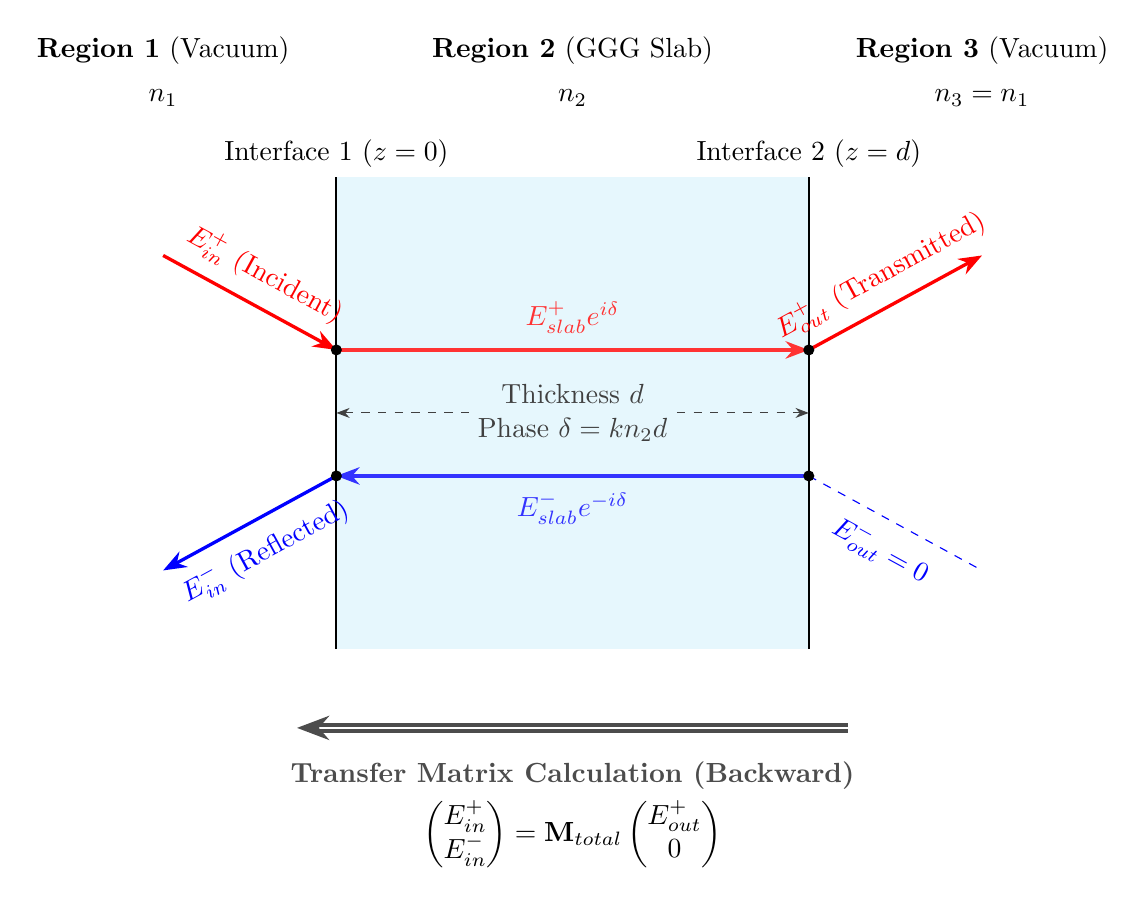
\begin{tikzpicture}[>=Stealth, scale=1.0]
        % --- 定義: サイズと配置の調整 ---
        \def\slabW{6.0}   
        \def\h{3.0}       
        \def\labelOffsetOne{1.6} 
        \def\labelOffsetTwo{1.0} 
        \def\textOffsetSide{2.2} 

        % --- 領域ラベル (最上段) ---
        \node at (-\textOffsetSide, \h+\labelOffsetOne) {\textbf{Region 1} (Vacuum)};
        \node at (\slabW/2, \h+\labelOffsetOne) {\textbf{Region 2} (GGG Slab)};
        \node at (\slabW+\textOffsetSide, \h+\labelOffsetOne) {\textbf{Region 3} (Vacuum)};

        % --- 屈折率 (中段) ---
        \node at (-\textOffsetSide, \h+\labelOffsetTwo) {$n_1$};
        \node at (\slabW/2, \h+\labelOffsetTwo) {$n_2$};
        \node at (\slabW+\textOffsetSide, \h+\labelOffsetTwo) {$n_3 = n_1$};

        % --- スラブと界面の描画 ---
        \fill[cyan!10] (0, -\h) rectangle (\slabW, \h);
        
        \draw[thick] (0, -\h) -- (0, \h);
        \node[above] at (0, \h) {Interface 1 ($z=0$)}; 
        
        \draw[thick] (\slabW, -\h) -- (\slabW, \h);
        \node[above] at (\slabW, \h) {Interface 2 ($z=d$)};
        
        % --- 電場ベクトル ---
        % 入射・反射 (Region 1)
        \draw[->, very thick, red] (-\textOffsetSide, 2.0) -- (0, 0.8) node[midway, above, sloped, yshift=2pt] {$E_{in}^+$ (Incident)};
        \draw[<-, very thick, blue] (-\textOffsetSide, -2.0) -- (0, -0.8) node[midway, below, sloped, yshift=-2pt] {$E_{in}^-$ (Reflected)};
        
        % 内部多重反射 (Region 2)
        \draw[->, very thick, red!80] (0, 0.8) -- (\slabW, 0.8) node[midway, above, yshift=2pt] {$E_{slab}^+ e^{i\delta}$};
        \draw[<-, very thick, blue!80] (0, -0.8) -- (\slabW, -0.8) node[midway, below, yshift=-2pt] {$E_{slab}^- e^{-i\delta}$};
        
        % 位相シフト表示
        \draw[<->, dashed, darkgray] (0, 0) -- (\slabW, 0) node[midway, fill=cyan!10, align=center, inner sep=3pt] {Thickness $d$ \\ Phase $\delta=kn_2d$};

        % 透過 (Region 3)
        \draw[->, very thick, red] (\slabW, 0.8) -- (\slabW+\textOffsetSide, 2.0) node[midway, above, sloped, yshift=2pt] {$E_{out}^+$ (Transmitted)};
        \draw[dashed, blue] (\slabW, -0.8) -- (\slabW+\textOffsetSide, -2.0) node[midway, below, sloped, yshift=-2pt] {$E_{out}^- = 0$};

        % --- 行列演算の概念図 (下部) ---
        \draw[<-, double, line width=1.5pt, black!70] (-0.5, -4.0) -- (\slabW+0.5, -4.0) node[midway, below=8pt, font=\bfseries] {Transfer Matrix Calculation (Backward)};
        
        \node[anchor=north] at (\slabW/2, -4.8) {
            $\displaystyle \begin{pmatrix} E_{in}^+ \\ E_{in}^- \end{pmatrix} = \mathbf{M}_{total} \begin{pmatrix} E_{out}^+ \\ 0 \end{pmatrix}$
        };

        % --- 結合点の黒丸 ---
        \foreach \x/\y in {0/0.8, 0/-0.8, \slabW/0.8, \slabW/-0.8}
            \fill[black] (\x, \y) circle (2pt);

    \end{tikzpicture}
    
    % --- キャプションとラベル ---
    \caption{転送行列法によるGGGの多層構造の計算モデル\\屈折率\(n_1, n_2, n_3\)および厚さ\(d\)を持つGGGスラブを通過する電磁波の伝搬を解析するためのモデル図. 各界面での入射波、反射波、透過波、およびスラブ内部での多重反射波を示している. また, 下部には転送行列計算の概念図を示し, 入射波と透過波の関係を行列形式で表現していることを強調している.}
    \label{fig:ggg_tmm_model}
\end{figure}

\subsection{問題設定}
\begin{itemize}
    \item \textbf{領域 1 (左側)}: 真空 (\(n_1 = 1\))
    \item \textbf{領域 2 (薄膜)}: GGG (\(n_2\), 厚さ \(d\))
    \item \textbf{領域 3 (右側)}: 真空 (\(n_3 = n_1 = 1\))
\end{itemize}

\subsection{転送行列の定式化 (Backward Definition)}
数学的な整合性を保つため, 標準的な光学テキスト(Born \& Wolf等)で採用されている\textbf{Backward転送行列}を使用する. これは, 出力側(右側)の場から入力側(左側)の場を逆算する形式である. 
\begin{equation}
    \begin{pmatrix} E_{in}^+ \\ E_{in}^- \end{pmatrix} = \mathbf{M}_{total} \begin{pmatrix} E_{out}^+ \\ E_{out}^- \end{pmatrix}
\end{equation}
ここで, \(E^+\) は進行波, \(E^-\) は後退波を表す. 透過問題を考えるため, スラブのさらに右側からの入射はないものとし, 境界条件 \(E_{out}^- = 0\) を課す. 

透過係数 \(t_{slab}\) および反射係数 \(r_{slab}\) は以下のように定義される. 
\begin{equation}
    t_{slab} = \frac{E_{out}^+}{E_{in}^+} = \frac{1}{(\mathbf{M}_{total})_{11}}, \quad r_{slab} = \frac{E_{in}^-}{E_{in}^+} = \frac{(\mathbf{M}_{total})_{21}}{(\mathbf{M}_{total})_{11}}
\end{equation}

\subsubsection*{構成行列}

\textbf{1. 界面行列(媒質 \(i \to j\)):}
フレネル係数を用いると, 界面における場の接続行列は以下のようになる. 
\begin{equation}
    \mathbf{M}_{ij} = \frac{1}{t_{ij}} \begin{pmatrix} 1 & r_{ij} \\ r_{ij} & 1 \end{pmatrix}
\end{equation}
ここで, 垂直入射におけるフレネル係数は次式で与えられる. 
\begin{equation}
    r_{ij} = \frac{n_i - n_j}{n_i + n_j}, \quad t_{ij} = \frac{2n_i}{n_i + n_j}
\end{equation}
対称性 \(r_{ji} = -r_{ij}\) およびストークスの関係式 \(t_{ij}t_{ji} = 1 - r_{ij}^2\) が成立することに注意する. 

\textbf{2. 伝搬行列(媒質 \(j\) 内部):}
厚さ \(d\) の媒質内部での位相シフトを \(\delta = k_0 n_j d\) とする. 位置 \(z+d\) から \(z\) へ逆算する伝搬行列は以下の通りである. 
\begin{equation}
    \mathbf{M}_{prop} = \begin{pmatrix} e^{-i\delta} & 0 \\ 0 & e^{i\delta} \end{pmatrix}
\end{equation}
(注:物理的な進行波 \(E^+\) は前方へ進むにつれ \(e^{i\delta}\) の位相を獲得する. したがって, 出力側から入力側へ「戻る」計算を行うBackward行列では, 逆位相 \(e^{-i\delta}\) を乗じる必要がある. )
\subsection{全行列の計算}
「真空 \(\to\) GGG \(\to\) 真空」系の全転送行列は, 物理的な配置の逆順に行列を掛け合わせることで得られる. 
\begin{equation}
    \mathbf{M}_{GGG} = \mathbf{M}_{12} \cdot \mathbf{M}_{prop} \cdot \mathbf{M}_{21}
\end{equation}
成分を代入して計算する. 
\begin{align}
    \mathbf{M}_{GGG} &= \frac{1}{t_{12}} \begin{pmatrix} 1 & r_{12} \\ r_{12} & 1 \end{pmatrix}
    \begin{pmatrix} e^{-i\delta} & 0 \\ 0 & e^{i\delta} \end{pmatrix}
    \frac{1}{t_{21}} \begin{pmatrix} 1 & r_{21} \\ r_{21} & 1 \end{pmatrix} \\
    &= \frac{1}{t_{12}t_{21}} \begin{pmatrix} 1 & r_{12} \\ r_{12} & 1 \end{pmatrix}
    \begin{pmatrix} e^{-i\delta} & r_{21} e^{-i\delta} \\ r_{21} e^{i\delta} & e^{i\delta} \end{pmatrix}
\end{align}
ここで, \(r_{21} = -r_{12} \equiv -r\) と置き, 透過係数の導出に必要な \((1,1)\) 成分のみを計算する. 
\begin{align}
    (\mathbf{M}_{GGG})_{11} &= \frac{1}{t_{12}t_{21}} \left[ 1 \cdot (e^{-i\delta}) + r_{12} \cdot (r_{21} e^{i\delta}) \right] \\
    &= \frac{1}{1 - r^2} \left( e^{-i\delta} - r^2 e^{i\delta} \right)
\end{align}
ここでは恒等式 \(t_{12}t_{21} = 1 - r^2\) を用いた. 

\subsection{透過係数の導出と結論}
スラブ全体の透過係数は次式で求まる. 
\begin{equation}
    t_{slab} = \frac{1}{(\mathbf{M}_{GGG})_{11}} = \frac{1 - r^2}{e^{-i\delta} - r^2 e^{i\delta}}
\end{equation}

標準的なファブリ・ペローの公式と比較するため, 分母・分子に \(e^{i\delta}\) を乗じて整理する. 
\begin{equation}
    t_{slab} = \frac{(1 - r^2) e^{i\delta}}{1 - r^2 e^{2i\delta}}
\end{equation}
ここで, \(\delta = n_2 k_0 d = \frac{2\pi n_2 d}{\lambda}\) である. 

\subsubsection*{インピーダンス\(Z\)による表現}
この式を, インピーダンスパラメータ \(Z\)(ただし \(r = \frac{1-Z}{1+Z}\), \(Z=\sqrt{\frac{\mu_{r}}{\epsilon_{r}}}\))を用いて書き直すと以下のようになる. 
\begin{equation}
    t_{slab} = \frac{ \frac{4Z}{(1+Z)^2} e^{i\delta} }{ 1 - \left(\frac{1-Z}{1+Z}\right)^2 e^{2i\delta} } 
    = \frac{4Z e^{i\delta}}{(1+Z)^2 - (1-Z)^2 e^{2i\delta}}
\end{equation}
\section{ベイズ推定}
\label{sec:method_bayesian}
物理実験, 特にGGGの分光測定のような複雑な系においては, 観測データにノイズが含まれるだけでなく, 理論モデル自体にも不確実性が存在する. 従来の最小二乗法(最尤推定)による点推定では, パラメータ間の相関や多峰性を捉えきれず, 過学習のリスクも高い. 本章では, これらの問題を解決し, 厳密な不確実性評価を可能にするベイズ推論の枠組みを詳述する. 
\subsubsection{ベイズの定理}
ベイズ推定は, 観測データ \(D\) に基づいてモデルパラメータ \(\theta\) の確率分布を更新する枠組みである. ベイズの定理により, 事後分布 \(p(\theta|D)\) は以下のように表される.
\begin{equation}
p(\theta|D) = \frac{\mathcal{L}(\theta | D) p(\theta)}{p(D)} \label{equation_bayesian}
\end{equation}
ここで, \(\mathcal{L}(\theta | D)\) (=\(p(D|\theta)\))は尤度関数, \(p(\theta)\) は事前分布, \(p(D)\) は周辺尤度(正規化定数)である. ベイズ推定の目的は, 観測データに基づいてパラメータの不確実性を反映した事後分布を得ることである.
\subsubsection*{事前分布}
事前分布 \(p(\theta)\) は, 観測データを得る前のパラメータに関する知識や仮定を反映する. 例えば, 物理的制約や過去の研究結果に基づいて, パラメータが特定の範囲にあることを示す一様分布や, より具体的な情報を反映した正規分布などが用いられる.
本研究の解析においては, g因子に対して, ランデのg因子を平均とした正規分布を設定したり, あるいは物理的に取りうる範囲(正値性など)を正規分布として与えたりする. 事前分布は, 推定の「正則化」として機能し, データが少ない場合でも非物理的な解への発散を防ぐ役割を果たす. 
\subsubsection*{尤度関数}
尤度関数 \(\mathcal{L}(\theta | D)\) は, パラメータ \(\theta\) のもとで観測データ \(D\) が得られる確率を表す. 通常, 観測データのノイズモデルに基づいて定義される. 例えば, 観測誤差が正規分布に従う場合, 尤度関数は以下のように表される.
\begin{equation}
\mathcal{L}(\theta | D) = \prod_{i} \frac{1}{\sqrt{2\pi \sigma^2}} \exp\left( -\frac{(D_i - f(x_i; \theta))^2}{2\sigma^2} \right)
\end{equation}
ここで, \(f(x_i; \theta)\) はモデル関数, \(\sigma\) は観測ノイズの標準偏差である. 尤度関数は, 観測データとモデル予測の一致度を定量化し, パラメータ推定において重要な役割を果たす.

\subsubsection*{周辺尤度}
周辺尤度 \(p(D)\) は, 観測データ \(D\) が得られる全確率を表し, 事後分布の正規化定数として機能する. これは, 全てのパラメータ空間にわたる尤度関数と事前分布の積分によって計算される.
\begin{equation}
    p(D) = \int \mathcal{L}(\theta | D) p(\theta) d\theta
\end{equation}
これは, パラメータ空間全体にわたって「モデルがデータを生成する平均的な能力」を積分した値である. モデル選択において極めて重要な指標であり, 例えば「H形式」と「B形式」のどちらがデータをより良く説明するかを比較する際の「ベイズ因子(Bayes Factor)」の算出に用いられる.
\subsubsection*{事後分布}
事後分布 \(p(\theta|D)\) は, 式\ref{equation_bayesian}にあるように, 観測データに基づいて更新されたパラメータの確率分布を表す. 事後分布は, 事前分布と尤度関数の積に比例し, 正規化定数 \(p(D)\) によって正規化される. 
事後分布からは, パラメータの最頻値(MAP推定値), 平均値, 分散などの統計量を計算できる.
ベイズ推論のゴールは, この事後分布の形状(平均, 分散, 相関構造など)を明らかにすることである. しかし, GGGのモデルのようにパラメータが多数存在し, モデルが非線形である場合, 事後分布を解析的に求めることは事実上不可能であり, 後述する数値計算手法(マルコフ連鎖モンテカルロ法など)が必要となる. 

\section{マルコフ連鎖モンテカルロ法}
\label{sec:method_mcmc}
ベイズ推定において, 事後分布 \(P(\theta|D)\) を直接計算することは困難であるため, マルコフ連鎖モンテカルロ法(MCMC)が広く用いられる. MCMCは, 事後分布から, その分布に従う乱数(サンプル)を効率的に生成するためのアルゴリズム群が, マルコフ連鎖モンテカルロ法(Markov Chain Monte Carlo: MCMC)である.
本節では, MCMCの基本的な考え方とアルゴリズムについて説明する.

\subsection{メトロポリス法}
最も古典的かつ基本的なMCMCアルゴリズムの一つに, メトロポリス法がある. メトロポリス法は, 事後分布 \(P(\theta|D)\) に比例する確率分布からサンプルを生成するための手法である. アルゴリズムの概要は以下の通りである.
\begin{enumerate}
    \item 初期状態 \(\theta_0\) を設定する.
    \item 現在の状態 \(\theta_t\) から新しい候補状態 \(\theta^*\) を提案する. 通常, 対称な提案分布 \(q(\theta^*|\theta_t)\)(例: 正規分布)を用いる.
    \item 受容確率 \(\alpha\) を計算する:
    \begin{equation}
        \alpha = \min\left(1, \frac{P(D|\theta^*) P(\theta^*)}{P(D|\theta_t) P(\theta_t)}\right)
    \end{equation}
    \item 一様乱数 \(u \sim U(0,1)\) を生成し, \(u < \alpha\) ならば新しい状態を受容し, \(\theta_{t+1} = \theta^*\) とする. そうでなければ, 現在の状態を維持し, \(\theta_{t+1} = \theta_t\) とする.
    \item ステップ2から4を繰り返し, 十分な数のサンプルを収集する.
\end{enumerate}
この手法は実装が容易であるが, パラメータ間の相関が強い場合や高次元空間では, 提案された候補の多くが棄却されるか, あるいはランダムウォーク的な挙動に陥り, 効率的にサンプリングできないことがある.

\subsection{スライスサンプリング}
スライスサンプリングは, メトロポリス法の欠点を克服するために開発されたMCMCアルゴリズムである. メトロポリス法における「ステップ幅(提案分布の分散)」の調整問題を解決するために, Nealによって考案された手法である\(^{\cite{Neal2003}}\).アルゴリズムの概要は以下の通りである.
\begin{enumerate}
    \item 初期状態 \(\theta_0\) を設定する.
    \item 現在の状態 \(\theta_t\) における事後分布の値 \(P(\theta_t|D)\) を計算し, 水平線の高さ \(y\) を一様乱数 \(u \sim U(0, P(\theta_t|D))\) によって決定する.
    \item 水平線 \(y\) と交わる事後分布の区間(スライス)を見つける.
    \item スライス内から新しい候補状態 \(\theta^*\) を一様にサンプリングする.
    \item 新しい状態を受容し, \(\theta_{t+1} = \theta^*\) とする.
    \item ステップ2から5を繰り返し, 十分な数のサンプルを収集する.
\end{enumerate}
このアルゴリズムは, 事後分布の形状に適応的にサンプリングを行うことで, 高次元空間や相関の強いパラメータ空間でも効率的にサンプルを生成できる. 

\subsection{NUTS(No-U-Return Sampler)}
NUTS (No-U-Turn Sampler) は, ハミルトニアンモンテカルロ法 (HMC) を基盤とした現代のベイズ統計ソフトウェア(Stan, PyMCなど)で標準エンジンとなっている最先端アルゴリズムである. \(^{\cite{Hoffman2014}}\)HMCは, 物理学のハミルトニアン力学系の概念を利用して, パラメータ空間を効率的に探索する手法であり, 以下に概要を示す. 
\subsubsection*{HMCの基礎}
HMCは, パラメータ \(\theta\) に対して仮想的な運動量 \(p\) を導入し, ハミルトニアン \(H(\theta, p) = U(\theta) + K(p)\) を定義する. ここで, \(U(\theta) = -\log P(\theta|D)\) はポテンシャルエネルギー, \(K(p) = \frac{1}{2} p^T M^{-1} p\) は運動エネルギーであり, \(M\) は質量行列である. HMCは, レヴィ・カンター方程式に基づいて \((\theta, p)\) の時間発展をシミュレートし, 新しい候補状態を生成する. この方法により, 高次元空間でも効率的にサンプリングが可能となる.
\subsubsection*{NUTSの革新性}
HMCの最大の課題は, 積分ステップ数\(L\)の調整である. \(L\)が短すぎるとランダムウォークになり, 長すぎると軌道が一周して元の位置に戻ってしまい(Uターン), 計算資源を浪費する. 
NUTSは, 以下の手順でこれを自動化する:
\begin{enumerate}
    \item \textbf{再帰的な二分木の構築}: ハミルトニアン力学系のシミュレーションを前進と後退の両方向に行い, ツリー構造を再帰的に構築する.
    \item \textbf{No-U-Turn停止条件の判定}: 構築された軌道の始点\(\theta^-\)と終点\(\theta^+\)を結ぶベクトルと, 終点の運動量ベクトル\(r^+\)の内積を確認する. これが負になった(\(( \theta^+ - \theta^- ) \cdot r^+ < 0\)), すなわち粒子が来た道を戻り始めた時点で, 木の拡張を停止する.
    \item \textbf{詳細釣り合いの維持}: 新しい候補状態を選択する際に, 停止位置までの軌道上の点から, スライスサンプリングの考え方を応用して次の点を抽出する.これにより, 詳細釣り合い条件を満たすように確率的に選択を行う.
\end{enumerate}
これにより, 高次元かつ相関の強いGGGの結晶場パラメータ空間においても, 極めて高い効率(有効サンプルサイズの最大化)で事後分布を探索することが可能となる. 

\section{LOO-CV(Leave-One-Out Cross-Validation)}
\label{sec:method_loo_cv}
ベイズモデルの予測性能を評価し, 過学習を防ぐための主要な手法として, 1個抜き交差検証(Leave-One-Out Cross-Validation: LOOCV)がある\(^{\cite{Stone1974LOO}}\). 
LOOCVは, 観測データセット \(D = \{(x_i, y_i)\}_{i=1}^{N}\) に対して, 各データ点を一つずつ検証用データとして取り除き, 残りのデータでモデルを学習し, 取り除いたデータ点に対する予測性能を評価する手法である. 具体的な手順は以下の通りである.
\begin{enumerate}
    \item データセット \(D\) から, 各データ点 \((x_i, y_i)\) を一つずつ取り除き, 検証用データセット \(D_{-i} = D \setminus \{(x_i, y_i)\}\) を作成する.
    \item 検証用データセット \(D_{-i}\) を用いてモデルを学習し, 事後分布 \(P(\theta|D_{-i})\) を得る.
    \item 学習したモデルを用いて, 取り除いたデータ点 \((x_i, y_i)\) に対する予測分布 \(P(y_i|x_i, D_{-i})\) を計算する.
    \item 予測性能を評価するために, 例えば対数尤度を用いて次式のように計算する.
    \begin{equation}
        \text{LOO-CV} = \frac{1}{N} \sum_{i=1}^{N} \log P(y_i|x_i, D_{-i})
    \end{equation}
\end{enumerate}
LOOCVは, データセット全体を用いたモデルの汎化性能を評価するための厳密な方法であり, 特にデータ数が少ない場合に有効である. しかし, 各データ点ごとにモデルを再学習する必要があるため, 計算コストが高くなる欠点もある. そのため, 実際の応用では, 近似的な手法(例えば, WAICやPSIS-LOOなど)を用いることも検討される. 本研究でも, モデル比較の際は, 計算効率を考慮してArvizライブラリで実装されているPSIS-LOOを採用した.
\subsubsection*{PSIS-LOOによる高速化}
PSIS-LOO (Pareto Smoothed Importance Sampling Leave-One-Out) は, LOOCVの計算コストを大幅に削減するための近似手法である\(^{\cite{Vehtari2017}}\). 単純なLOOCVは, データ点数\(N\)回分のMCMC実行を要し, 計算コストが膨大である. そこで, 全データを用いた事後分布\(p(\theta | y)\)からのサンプル\(\theta^s\)を利用して, \(p(\theta | y_{-i})\)を近似する重点サンプリング(Importance Sampling: IS)が用いられる. 
ISの重みは \(w_i^s \propto 1 / p(y_i | \theta^s)\) となるが, この重みの分散はしばしば発散し, 推定が不安定になる. 
PSIS (Pareto Smoothed Importance Sampling)は, この重み分布の裾を一般化パレート分布で近似・平滑化することで, 分散を劇的に低減させる. 推定されたパレート分布の形状パラメータ\(k\)は, 近似の信頼性を診断する指標としても機能する(\(k < 0.7\)なら信頼できる). 
この手法により, 1回のMCMCシミュレーションの結果のみを用いて, 厳密なLOOCVとほぼ同等の精度でモデル評価・比較を行うことが可能となり, GGGのハミルトニアンモデル選択において強力なツールとなる. 
% chapters/method.tex の中身

\chapter{解析方法}
\label{chap:method} % 後で参照するためにラベルを付ける

本研究では, 取得されたTHz帯透過スペクトルの解析にあたり, 物理モデルに基づくパラメータ推定を行う. 解析は三段階で構成される. 第一に, 重み付き非線形最小二乗法を用いて大域的な最適解近傍を探索し, 第二に, その結果を事前情報として組み込んだベイズ推定を行うことで, パラメータの不確実性と相関を評価する. 第三に, WAIC及びPSISを用いたLOOCVにより, モデルの汎化性能を2つの情報規準に基づき評価する. 以下, 各手法の詳細について述べる.

\section{各準位の緩和係数}
磁気感受率は式\ref{eq:chi_linear}によって計算される. GGGは8準位あるので, 全\(8 \times 7 = 56\)個の遷移ペア( \(n \leftrightarrow n'\) )の寄与を考える必要がある. 計算コストの観点から, 本研究では, 式\ref{eq:gamma_approximation}を仮定し, 表\ref{tab:gamma_transition}で示すように, 56個の遷移の緩和係数を7個の緩和係数で記述する. 以下, この仮定に基づく緩和係数を共有\(\gamma\)モデルと呼称する. 
\begin{equation}
    \gamma (n, n') = \gamma_{\text{min}} (n, n')
    \label{eq:gamma_approximation}
\end{equation}
この物理的意味は, 緩和過程が主に初期状態(低エネルギー側)の特性で決まるという仮定である. 
\begin{table}[htbp]
\centering
\caption{共有\(\gamma\)モデル}
\begin{tabular}{lcccc}
\toprule
\textbf{\(\gamma_{i}\)} & \textbf{遷移パターン} & \textbf{遷移数}\\
\midrule
\(\gamma_0\) & \(|0\rangle \leftrightarrow |1,2,\dots,7\rangle\) & \(7 \times 2 = 14\)\\
\(\gamma_1\) & \(|0\rangle \leftrightarrow |2, \dots,7\rangle\) & \(6 \times 2 = 12\)\\
\(\gamma_2\) & \(|0\rangle \leftrightarrow |3, \dots,7\rangle\) & \(5 \times 2 = 10\)\\
\(\gamma_3\) & \(|0\rangle \leftrightarrow |4,\dots,7\rangle\) & \(4 \times 2 =8\)\\
\(\gamma_4\) & \(|0\rangle \leftrightarrow |5,\dots,7\rangle\) & \(3 \times 2 = 6\)\\
\(\gamma_5\) & \(|0\rangle \leftrightarrow |6,7\rangle\) & \(2 \times 2 = 4\)\\
\(\gamma_6\) & \(|0\rangle \leftrightarrow |7 \rangle\) & \(1 \times 2 = 2\)\\
\bottomrule
\end{tabular}
\label{tab:gamma_transition}
\end{table}

\section{推定するパラメータ群}
\label{sec:parameters_to_estimate}
本解析において推定対象となる主要なパラメータ群とその物理的役割を Table \ref{tab:parameters_1} にまとめる. 

\begin{table}[htbp]
    \centering
    \caption{本解析における推定パラメータ群とその物理的役割}
    \label{tab:parameters_1}
    \renewcommand{\arraystretch}{1.3} % 行の高さを調整
    \begin{tabular}{@{}llp{8.5cm}@{}}
        \toprule
        \textbf{記号} & \textbf{パラメータ名称} & \textbf{物理的役割とモデルへの寄与} \\
        \midrule
        \(g_{J}\) & g因子 & ゼーマンエネルギー \(\muB g_{J} B\) を決定し, スペクトルの共鳴中心周波数を支配する.  \\
        \(B_{4}, B_{6}\) & 結晶場パラメータ & ゼロ磁場分裂や準位の混合を引き起こし, ピークの微細構造(分裂幅)やポラリトンモードに寄与する. \\
        \(\gamma_{i}\) & 緩和係数 & 遷移の寿命 \(\tau = 1/\gamma\) に対応し, スペクトルの線幅(Lorentzian幅)を決定する. コヒーレンスの減衰や散乱過程を反映する.  \\
        \(a_{\vb*{scale}}\) & スケーリング係数 & 実効的なスピン密度や試料充填率に依存する吸収強度の絶対値を補正する係数. \(\chi \propto a_{\vb*{scale}} \cdot g^2\) の関係を持つ.  \\
        \(\varepsilon_{\vb*{bg}}\) & 背景誘電率 & 磁気共鳴以外のバックグラウンド透過率および高次の共振器モードを決定する.  \\
        \bottomrule
    \end{tabular}
\end{table}

\section{重み付き非線形最小二乗法}
\label{sec:wnlls}
本節では, スペクトルフィッティングに用いる重み付き非線形最小二乗法の詳細について述べる.
本研究におけるスペクトルフィッティングでは, モデルパラメータ \(\bm{\theta}\) に対する物理的な制約条件(正値性や上下限)の遵守に加え, スペクトル形状の重要な特徴(共鳴ピークやディップ構造等)を精度よく再現することが求められる. 
均等な重み付けでは, 信号強度の小さい領域やノイズの影響により, 主要な特徴のフィッティング精度が損なわれる可能性がある. そのため, 各データ点の重要度を任意に調整可能な\textbf{重み付き信頼領域反射法}(Weighted Trust Region Reflective algorithm: Weighted-TRF)\(^{\cite{Branch1999}}\)を採用した. 

\subsection{目的関数と制約条件}
観測データベクトルを \(\bm{y}^{\mathrm{obs}}\), モデル関数を \(\bm{f}(\bm{\theta})\) とする. 各データ点 \(i\) に対する重要度を示す重み係数を \(w_i\) とし, これを対角成分に持つ重み行列 \(\vb*{W} = \mathrm{diag}(w_1, \dots, w_N)\) を導入する. 
目的関数 \(S(\bm{\theta})\) は, この重み行列を用いた重み付き残差二乗和として定義される. 
\begin{equation}
    \min_{\bm{\theta}} S(\bm{\theta}) = \frac{1}{2} \left( \bm{y}^{\mathrm{obs}} - \bm{f}(\bm{\theta}) \right)^T \vb*{W} \left( \bm{y}^{\mathrm{obs}} - \bm{f}(\bm{\theta}) \right)
    \label{eq:objective_function}
\end{equation}
ここで, 重み \(w_i\) はスペクトルの特徴的な領域(例えば透過率の変化が急峻な領域)に対して大きな値を設定することで, その領域のフィッティング優先度を高める役割を果たす. 
また, パラメータベクトル \(\bm{\theta}\) は以下の不等式制約を満たすものとする. 
\begin{equation}
    \bm{l} \le \bm{\theta} \le \bm{u}
    \label{eq:boundary_constraints}
\end{equation}
\(\bm{l}, \bm{u}\) はそれぞれパラメータの下限および上限ベクトルである. 

\subsection{信頼領域サブ問題と重み付きスケーリング}
Weighted-TRF法は反復解法であり, 第 \(k\) ステップにおけるパラメータ推定値 \(\bm{\theta}_k\) の近傍(信頼領域)において, 目的関数 \(S(\bm{\theta})\) を二次近似したモデル \(m_k(\bm{p})\) を最小化する探索ベクトル \(\bm{p}\) を決定する. 
\begin{equation}
    m_k(\bm{p}) = S(\bm{\theta}_k) + \vb*{g}_k^T \bm{p} + \frac{1}{2} \bm{p}^T \vb*{H}_k \bm{p}
    \label{eq:quadratic_model}
\end{equation}
ここで, 重み付き勾配ベクトル \(\vb*{g}_k\) およびガウス・ニュートン近似を用いた重み付きヘッセ行列 \(\vb*{H}_k\) は, ヤコビ行列 \(\vb*{J}_k\) を用いて以下のように記述される. 
\begin{equation}
    \vb*{g}_k = -\vb*{J}_k^T \vb*{W} (\bm{y}^{\mathrm{obs}} - \bm{f}(\bm{\theta}_k)), \quad \vb*{H}_k \approx \vb*{J}_k^T \vb*{W} \vb*{J}_k
\end{equation}
重み行列 \(\vb*{W}\) の導入により, 重要度の高いデータ点での残差を優先的に減少させる探索方向が選択される. 

\subsection{Levenberg-Marquardt法との比較}
一般に非線形最小二乗法の標準解法として知られるLevenberg-Marquardt法\(^{\cite{More1978}}\)は, ダンピング係数 \(\lambda\) を用いて最急降下法とガウス・ニュートン法を補間する強力な手法であるが, 本質的には制約なし問題を対象としている. LM法で境界条件を扱う場合, 変数のクリッピングやペナルティ関数などのヒューリスティックな処理が必要となり, 数値的な不安定性を招く恐れがある. 

\subsection{フィッティング手法とプログラムの全体フロー}    
\label{subsec:wnlls_method}
まず, Kritzellらの実験データを読み込み, 磁場・温度ごとにデータを分割する. 次に, 各モデル(H形式, B形式)について, 手作業でフィッティングした際の知見を活かした初期パラメータを設定し, 重み付き非線形最小二乗法を適用してフィッティングを行う. フィッティングには\texttt{Scipy}ライブラリの\texttt{optimize}モジュールに含まれる\texttt{least\_squares}関数を使用し, 各パラメータの最適値と共分散行列を取得する. 最後に, フィッティング結果を用いて各準位のエネルギー固有値と占有確率, 磁気感受率, 透過スペクトルを算出し, 結果を保存する. 重み付け方法としては, ピーク検出アルゴリズムにより特定された共鳴中心周波数および半値全幅(FWHM)内の領域に対して大きな値を与え, それ以外の領域には小さな値を与える. ただし, ポラリトン形成領域のフィッティングが困難だった為, ポラリトン形成領域の方が高次共振器モードよりも高く設定した.
図\ref{fig:flowchart_wnlls}に, 重み付き非線形最小二乗法の全体フローチャートを示す. 初期条件は表\ref{tab:parameters_initial_wnlls}, フィッティング条件は表\ref{tab:stepwise_fitting_parameters}の通りである.サンプリング効率を向上させるため,各パラメータをスケーリングして最適化空間で同程度の変動幅を持つようにした:
\begin{equation}
    \theta_{\mathrm{scaled}} = \theta_{\mathrm{physical}} \times s_\theta
\end{equation}
スケーリング係数\(s_\theta\)を表\ref{tab:scaling}に示す.

\begin{table}[htbp]
\centering
\caption{重み付き非線形最小二乗法の全パラメータの初期条件}
\begin{tabular}{lcccc}
\toprule
\textbf{カテゴリ} & \textbf{パラメータ} & \textbf{初期値} & \textbf{範囲}\\
\midrule
\multirow{5}{*}{Global (5個)} 
 & \(g_{J}\) & 1.95 & [1.5, 2.8]\\
 & \(a\) & 1.0 & [0.1, 5.0]\\
 & \(B_4\) & 2.02 mK & [0.1, 30] mK\\
 & \(B_6\) & \(-0.012\) mK & [-1.0, 1.0] mK\\
 & \(\varepsilon_{\text{bg}}\) & 14.4 & [13.0, 16.0]\\
\midrule
\multirow{7}{*}{Shared \(\gamma\) (7個)} 
 & \(\gamma_0\) & 0.10 THz & [0.01, 0.5] THz\\
 & \(\gamma_1\) & 0.15 THz & [0.01, 0.5] THz\\
 & \(\gamma_2\) & 0.12 THz & [0.01, 0.5] THz\\
 & \(\gamma_3\) & 0.11 THz & [0.01, 0.5] THz\\
 & \(\gamma_4\) & 0.14 THz & [0.01, 0.5] THz\\
 & \(\gamma_5\) & 0.13 THz & [0.01, 0.5] THz\\
 & \(\gamma_6\) & 0.16 THz & [0.01, 0.5] THz\\
\bottomrule
\end{tabular}
\label{tab:parameters_initial_wnlls}
\end{table}

\begin{table}[htbp]
    \centering
    \caption{\textbf{重み付き非線形最小二乗法の段階的フィッティング条件}}
    \label{tab:stepwise_fitting_parameters}
    \renewcommand{\arraystretch}{1.2} % 行間調整
    \begin{tabular}{@{}lccc@{}}
        \toprule
        \multicolumn{4}{c}{\textbf{段階的最適化設定}} \\
        \cmidrule(lr){1-4}
        \textbf{パラメータ項目} & \textbf{Stage 1} & \textbf{Stage 2} & \textbf{Stage 3} \\
        & (粗探索) & (中間精緻化) & (微調整) \\
        \midrule
        最大反復回数 (\(N_{\text{max}}\)) & 5,000 & 15,000 & 30,000 \\
        関数値収束許容誤差 (\texttt{ftol}) & \(1.0 \times 10^{-5}\) & \(1.0 \times 10^{-7}\) & \(1.0 \times 10^{-9}\) \\
        パラメータ収束許容誤差 (\texttt{xtol}) & \(1.0 \times 10^{-5}\) & \(1.0 \times 10^{-7}\) & \(1.0 \times 10^{-9}\) \\
        \midrule
        \multicolumn{4}{c}{\textbf{共通設定}} \\
        \cmidrule(lr){1-4}
        \multicolumn{2}{l}{最適化アルゴリズム} & \multicolumn{2}{l}{TRF法} \\
        \multicolumn{2}{l}{ポラリトンモードの重み (\(w_{\text{pol}}^{\text{WNLLS}}\))} & \multicolumn{2}{l}{1.5} \\
        \multicolumn{2}{l}{共振器モードの重み (\(w_{\text{cav}}^{\text{WNLLS}}\))} & \multicolumn{2}{l}{1.0} \\
        \multicolumn{2}{l}{背景・ノイズ領域の重み (\(w_{\text{bg}}^{\text{WNLLS}}\))} & \multicolumn{2}{l}{0.01} \\
        \bottomrule
    \end{tabular}
\end{table}

\begin{table}[htbp]
\centering
\caption{パラメータスケーリング係数}
\label{tab:scaling}
\begin{tabular}{lcc}
\toprule
パラメータ & スケーリング係数 \(s_\theta\) & スケール後の範囲 \\
\midrule
\(g_{J}\) & 38.0 & \([57, 106]\) \\
\(a\) & 10.2 & \([1.0, 102]\) \\
\(B_4\) & 1672.0 & \([0.017, 83.6]\) \\
\(B_6\) & 25000.0 & \([-50, 50]\) \\
\(\varepsilon_{\mathrm{bg}}\) & 17.0 & \([221, 272]\) \\
\(\gamma\) & 100.0 & \([0.5, 50]\) \\
\bottomrule
\end{tabular}
\end{table}

\begin{figure}[htbp]
\centering
\begin{tikzpicture}[
    node distance=1.2cm,
    startstop/.style={rectangle, rounded corners, minimum width=3cm, minimum height=0.8cm, text centered, draw=black, fill=red!30},
    process/.style={rectangle, minimum width=3cm, minimum height=0.8cm, text centered, draw=black, fill=orange!30},
    io/.style={trapezium, trapezium left angle=70, trapezium right angle=110, minimum width=3cm, minimum height=0.8cm, text centered, draw=black, fill=blue!30},
    decision/.style={diamond, minimum width=2cm, minimum height=0.8cm, text centered, draw=black, fill=green!30},
    arrow/.style={thick,->,>=stealth}
]

% ノード
\node (start) [startstop] {開始};
\node (load) [io, below of=start] {データロード (10セット)};
\node (detect) [process, below of=load] {ポラリトン検出・重み付け};
\node (init) [process, below of=detect] {初期値・境界値設定};
\node (opt1) [process, below of=init] {Stage 1: 粗探索};
\node (opt2) [process, below of=opt1] {Stage 2: 中間精緻化};
\node (opt3) [process, below of=opt2] {Stage 3: 微調整};
\node (analyze) [process, below of=opt3] {結果解析・診断};
\node (plot) [io, below of=analyze] {プロット生成・保存};
\node (end) [startstop, below of=plot] {終了};

% 矢印
\draw [arrow] (start) -- (load);
\draw [arrow] (load) -- (detect);
\draw [arrow] (detect) -- (init);
\draw [arrow] (init) -- (opt1);
\draw [arrow] (opt1) -- (opt2);
\draw [arrow] (opt2) -- (opt3);
\draw [arrow] (opt3) -- (analyze);
\draw [arrow] (analyze) -- (plot);
\draw [arrow] (plot) -- (end);

% モデル形式のループ
\node[draw, dashed, fit=(opt1)(opt2)(opt3)(analyze), inner sep=0.3cm, label=right:{\small H形式・B形式で繰り返し}] {};

\end{tikzpicture}
\caption{プログラムの処理フロー}
\label{fig:flowchart_wnlls}
\end{figure}
\clearpage

\section{重み付き尤度に基づくベイズ推定}
\label{sec:weighted_bayesian}
点推定である最小二乗法に対し, パラメータの事後確率分布 \(p(\vb*{\theta} | D)\) を求めることで, 推定値の不確実性とパラメータ間の相関を定量化する. 

\subsection{尤度関数の設計}
\label{subsec:likelihood}

観測透過率\(T_{\mathrm{obs},i}\)とモデル予測透過率\(T_{\mathrm{model},i}(\bm{\theta})\)の残差分布として,
外れ値に頑健なStudent-t分布を採用した\(^{\cite{Lange1989}}\):
\begin{equation}
    T_{\mathrm{obs},i} \sim \mathrm{StudentT}\left(\nu, T_{\mathrm{model},i}(\bm{\theta}), \sigma_{\mathrm{eff},i}\right)
    \label{eq:studentt_likelihood}
\end{equation}
ここで,\(\nu = 4\)は自由度であり,正規分布よりも裾の重い分布を実現する.

\subsubsection{Student-t分布の定義と性質}

Student-t分布は1908年にW. S. Gosset(ペンネーム「Student」)によって導入された確率分布である\(^{\cite{Student1908}}\).
自由度\(\nu\),位置パラメータ\(\mu\),スケールパラメータ\(\sigma\)を持つStudent-t分布の確率密度関数は次式で定義される\(^{\cite{Gelman2013}}\):
\begin{equation}
    p(x|\nu, \mu, \sigma) = \frac{\Gamma\left(\frac{\nu+1}{2}\right)}{\Gamma\left(\frac{\nu}{2}\right)\sqrt{\pi\nu}\sigma}
    \left(1 + \frac{1}{\nu}\left(\frac{x-\mu}{\sigma}\right)^2\right)^{-\frac{\nu+1}{2}}
    \label{eq:studentt_pdf}
\end{equation}
ここで\(\Gamma(\cdot)\)はガンマ関数である.

Student-t分布は自由度\(\nu\)によって裾の重さが制御される:
\begin{itemize}
    \item \(\nu = 1\):\textbf{コーシー分布}に一致.平均・分散が定義されない極端に裾の重い分布.
    \item \(\nu = 4\):本研究で採用.平均が存在し(\(\nu > 1\)),分散も有限(\(\nu > 2\))だが,正規分布より裾が重い.
    \item \(\nu = 10\):正規分布に近づくが,まだ裾が重い.
    \item \(\nu \to \infty\):\textbf{正規分布}に収束.
\end{itemize}

自由度\(\nu\)が小さいほど裾が重くなり,外れ値の影響を受けにくくなる.
一方,\(\nu\)が小さすぎると推定効率が低下する.
Langeら\(^{\cite{Lange1989}}\)の研究に基づき,頑健性と効率性のトレードオフを考慮して\(\nu = 4\)を採用した.

Student-t分布の主要な統計量は以下の通りである:
\begin{align}
    \text{期待値} &: \quad \mathbb{E}[X] = \mu \quad (\nu > 1) \\
    \text{分散} &: \quad \mathrm{Var}[X] = \sigma^2 \frac{\nu}{\nu - 2} \quad (\nu > 2) \\
    \text{尖度} &: \quad \kappa = \frac{6}{\nu - 4} + 3 \quad (\nu > 4)
\end{align}

\(\nu = 4\)の場合,分散は\(2\sigma^2\)となり,正規分布の2倍の広がりを持つ.
また尖度は定義されない(\(\nu > 4\)が必要)が,これは裾の重さを反映している.

有効標準偏差\(\sigma_{\mathrm{eff},i}\)は重み付き誤差として次式で定義される:
\begin{equation}
    \sigma_{\mathrm{eff},i} = \frac{\sigma_0}{\sqrt{w_i}}
    \label{eq:sigma_eff}
\end{equation}
ここで\(\sigma_0 = 0.01\)は基準標準偏差,\(w_i\)は各データ点の重みである.

重みは物理的重要性に基づいて表\ref{tab:bayes_weights}のように設定した:
\begin{table}[htbp]
    \centering
    \caption{ベイズ推定における周波数領域ごとの重み付け定義}
    \label{tab:bayes_weights}
    \begin{tabular}{llcl}
        \toprule
        領域区分 & 周波数帯域 (\(f\)) & 重み (\(w^{\text{bayes}}\)) & 物理的解釈・備考 \\
        \midrule
        ポラリトン領域 & \(< 0.3615~\text{THz}\) & \(2.0\) & \begin{tabular}[t]{@{}l@{}}磁気ポラリトン形成の核心領域 \\ \footnotesize{(注: WNLLS値 \(1.5\) とは異なる値を採用)}\end{tabular} \\
        \addlinespace
        共振器モード領域 & \(> 0.45~\text{THz}\) & \(1.0\) & 高次Fabry-Pérot干渉モード \\
        \addlinespace
        その他の領域 & その他 & \(0.01\) & 背景領域(軽視) \\
        \bottomrule
    \end{tabular}
\end{table}

\subsection{サンプリング手法}
事後分布からのサンプリングには, 効率的なサンプリングが可能なSMC法を採用する. 

\subsection{ベイズ階層モデルの構築}
\label{sec:hierarchical_model}
\subsubsection{階層モデルの必要性}

7つの緩和係数パラメータ\(\gamma_1, \ldots, \gamma_7\)は個別に推定すると識別不能性の問題が生じる.
すなわち,異なる\(\gamma_i\)の組み合わせが同程度の尤度を与え,事後分布が多峰性を示す.
この問題を解決するため,\(\gamma_i\)を共通のハイパーパラメータから生成される階層モデルを採用した.

\subsubsection{Non-centered Parameterizationの導入}

階層モデルにおける「漏斗問題」を回避するため,Non-centered Parameterizationを採用した.

\textbf{Centered版}(従来法,収束性不良):
\begin{equation}
    \gamma_i \sim \mathcal{N}(\mu_\gamma, \sigma_\gamma)
\end{equation}

\textbf{Non-centered版}(本研究):
\begin{align}
    z_i &\sim \mathcal{N}(0, 1) \\
    \log\gamma_i &= \log\mu_\gamma + \log\sigma_\gamma \cdot z_i
    \label{eq:non_centered}
\end{align}

Non-centered版では標準正規変数\(z_i\)がハイパーパラメータと独立であるため,SMCサンプラーが効率的に事後分布を探索できる.

\subsubsection{事前分布の設定}
\label{subsec:priors}

各パラメータの事前分布は物理的制約に基づいて設定した.表\ref{tab:priors}に一覧を示す.ただし,表\ref{tab:scaling}と同様のスケーリング係数を適用し, 最適化空間で同程度の変動幅を持つようにした.また, HモデルとBモデルの事前分布図をそれぞれ図\ref{fig:prior_H},図\ref{fig:prior_B}にプロットする. また, HモデルとBモデルの事前分布図をそれぞれ図\ref{fig:prior_H},図\ref{fig:prior_B}にプロットする. 

\begin{table}[htbp]
    \centering
    \caption{ベイズモデルの事前分布設定}
    \label{tab:priors}
    \begin{tabular}{llcl}
        \toprule
        パラメータ & 分布型 & パラメータ & 物理的根拠 \\
        \midrule
        \(g_{J}\) & TruncatedNormal & \(\mu=2.0\), \(\sigma=0.05\), \([1.5, 2.8]\) & Gd\(^{3+}\)理論値 \\
        \addlinespace
        \(a\) & HalfNormal & \(\sigma=2.0\), \([0.1, 10.0]\) & 低値優先,正値制約 \\
        \addlinespace
        \(B_4\) & LogNormal & \(\mu_{\log}=\log(2\mathrm{mK})\), \(\sigma_{\log}=1.2\) & 正値制約,mKオーダー \\
        \addlinespace
        \(B_6\) & Normal & \(\mu=0\), \(\sigma=0.5\mathrm{mK}\), \([-2, +2]\mathrm{mK}\) & ゼロ中心対称 \\
        \addlinespace
        \(\varepsilon_{\mathrm{bg}}\) & TruncatedNormal & \(\mu=14.0\), \(\sigma=0.3\), \([13, 16]\) & 実験値\(^{\cite{Kritzell2024}}\)参照 \\
        \addlinespace
        \(\log\mu_\gamma\) & Normal & \(\mu=\log(0.074)\), \(\sigma=0.3\) & 最適化結果\footnotesize{(詳細は\ref{sec:wnlls_results}節.)} \\
        \addlinespace
        \(\log\sigma_\gamma\) & HalfNormal & \(\sigma=0.3\) & 正値制約 \\
        \addlinespace
        \(z_i\) (\(i=1,\ldots,7\)) & Normal & \(\mu=0\), \(\sigma=1\) & Non-centered基底 \\
        \bottomrule
    \end{tabular}
\end{table}

\begin{figure}[htbp]
    \centering
    \includegraphics[width=1.0\textwidth]{prior_distributions_H.png}
    \caption{H形式モデルの事前分布. 赤点線は重み付き非線形最小二乗法でのフィッティング値を示す.}
    \label{fig:prior_H}
\end{figure}

\begin{figure}[htbp]
    \centering
    \includegraphics[width=1.0\textwidth]{prior_distributions_B.png}
    \caption{B形式モデルの事前分布. 赤点線は重み付き非線形最小二乗法でのフィッティング値を示す.}
    \label{fig:prior_B}
\end{figure}

\subsection{プログラムの全体フロー}
図\ref{fig:flowchart_bayesian}にて, ベイズ推定を行うプログラムコードの全体フローチャートを示す. 
\begin{figure}[htbp]
\centering
\begin{tikzpicture}[
    node distance=1cm,
    startstop/.style={rectangle, rounded corners, minimum width=3cm, minimum height=0.7cm, 
                      text centered, draw=black, fill=red!30},
    process/.style={rectangle, minimum width=3.5cm, minimum height=0.7cm, 
                    text centered, draw=black, fill=orange!30},
    io/.style={trapezium, trapezium left angle=70, trapezium right angle=110, 
               minimum width=3cm, minimum height=0.7cm, text centered, draw=black, fill=blue!30},
    decision/.style={diamond, minimum width=2cm, minimum height=0.8cm, 
                     text centered, draw=black, fill=green!30},
    arrow/.style={thick,->,>=stealth}
]

\node (start) [startstop] {開始};
\node (loadv6) [io, below=of start] {v6最適化結果読み込み (H/B)};
\node (loaddata) [io, below=of loadv6] {実験データ読み込み (10セット)};
\node (weight) [process, below=of loaddata] {重み配列生成};

\node (modelH) [process, below left=1cm and 0.5cm of weight] {H形式モデル構築};
\node (modelB) [process, below right=1cm and 0.5cm of weight] {B形式モデル構築};

\node (smcH) [process, below=of modelH] {SMCサンプリング (H)};
\node (smcB) [process, below=of modelB] {SMCサンプリング (B)};

\node (save) [io, below=1.5cm of $(smcH)!0.5!(smcB)$] {結果保存 (trace, summary)};
\node (plot) [process, below=of save] {比較プロット生成};
\node (end) [startstop, below=of plot] {終了};

\draw [arrow] (start) -- (loadv6);
\draw [arrow] (loadv6) -- (loaddata);
\draw [arrow] (loaddata) -- (weight);
\draw [arrow] (weight) -| (modelH);
\draw [arrow] (weight) -| (modelB);
\draw [arrow] (modelH) -- (smcH);
\draw [arrow] (modelB) -- (smcB);
\draw [arrow] (smcH) |- (save);
\draw [arrow] (smcB) |- (save);
\draw [arrow] (save) -- (plot);
\draw [arrow] (plot) -- (end);

\end{tikzpicture}
\caption{プログラム全体のフローチャート}
\label{fig:flowchart_bayesian}
\end{figure}

\section{モデル比較と評価}
ベイズ推定により得られた事後分布を用いて, H形式モデルとB形式モデルの適合度を比較・評価する.
本研究では, WAICとPSIS-LOO-CVの両方を採用した. それぞれ表\ref{tab:model_comparison}に示す特徴があり,補完的に利用することでモデル選択の信頼性を高めることができる.
WAICのみ悪い場合は事後分布の形状に問題がある可能性があり, PSIS-LOO-CVのみ悪い場合は外れ値の影響が大きい可能性があることが示唆される.
\begin{table}[htbp]
\centering
\caption{モデル比較指標の特徴}
    \begin{tabular}{lcc}
        \toprule
        指標 & WAIC & PSIS-LOO-CV \\
        \midrule
        計算方法 & 事後分布の対数尤度の情報量基準 & LOOCVの厳密近似, Pareto \(k\)診断で評価 \\
        \addlinespace
        長所 & 計算が高速で容易 & 外れ値に頑健,過学習を抑制 \\
        \addlinespace
        短所 & 外れ値に敏感,過学習のリスク & 計算コストが高い \\
        \bottomrule
    \end{tabular}
    \label{tab:model_comparison}
\end{table}
\chapter{結果と考察}
\label{chap:results}

本章では, 本研究で得られた主要な結果について述べる. まず, 重み付き非線形最小二乗法によるパラメータ推定結果を示し(\ref{sec:wnls_results}節), 次にベイズ推定に基づくパラメータの不確実性評価とモデル比較結果を提示する(\ref{sec:bayes_results}節). 最後に, これらの結果に基づく物理的考察を行う(\ref{sec:discussion}節).
\section{実験データセット}
\begin{table}[h]
\centering
\caption{使用データセット(10条件)}
\begin{tabular}{lccc}
\toprule
\textbf{データセット} & \textbf{磁場 $B$ [T]} & \textbf{温度 $T$ [K]} & \textbf{パターン} \\
\midrule
4K & 9.0 & 4.0 & 温度変化 \\
10K & 9.0 & 10.0 & 温度変化 \\
20K & 9.0 & 20.0 & 温度変化 \\
30K & 9.0 & 30.0 & 温度変化 \\
4.2T & 4.2 & 1.5 & 磁場変化 \\
5T & 5.0 & 1.5 & 磁場変化 \\
6T & 6.0 & 1.5 & 磁場変化 \\
7T & 7.0 & 1.5 & 磁場変化 \\
8T & 8.0 & 1.5 & 磁場変化 \\
9T & 9.0 & 1.5 & 磁場変化 \\
\bottomrule
\end{tabular}
\end{table}

\section{重み付き非線形最小二乗法によるパラメータ推定}
\label{sec:wnls_results}
まず, Kritzellらの実験データ\(^{\cite{Kritzell2024}}\)に対して重み付き非線形最小二乗法を適用し, H形式とB形式, それぞれのモデルのパラメータをフィッティングした. このフィッティングパラメータに基づき, 各準位のエネルギー固有値と占有確率, 磁気感受率, 透過スペクトルを算出した結果を以下に示す.

\subsection*{フィッティングパラメータの結果}
\label{subsec:wnlls_parameters}
\begin{table}[htbp]
    \centering
    \caption{共有$\gamma$モデルにおける最適化パラメータおよび評価指標の比較}
    \label{tab:parameters_results_wnlls}
    \renewcommand{\arraystretch}{1.2} % 行間の調整
    \begin{tabular}{@{}lcc@{}}
        \toprule
        \textbf{Parameter} & \textbf{Model H (H-form)} & \textbf{Model B (B-form)} \\
        \midrule
        \multicolumn{3}{@{}l@{}}{\textit{Global Parameters}} \\
        \quad $g$-factor ($g$) & 1.925 & 2.086 \\
        \quad Scaling factor ($a$) & 5.000 & 5.000 \\
        \quad Crystal field $B_4$ & $3.000 \times 10^{-2}$ & $1.592 \times 10^{-4}$ \\
        \quad Crystal field $B_6$ & $-1.000 \times 10^{-3}$ & $-9.989 \times 10^{-4}$ \\
        \quad Permittivity ($\epsilon$) & 14.001 & 14.131 \\
        \midrule
        \multicolumn{3}{@{}l@{}}{\textit{Shared Relaxation Rates ($\gamma_k$)}} \\
        \quad $\gamma_1$ & 0.0245 & 0.0237 \\
        \quad $\gamma_2$ & 0.0130 & 0.1445 \\
        \quad $\gamma_3$ & 0.1159 & 0.1148 \\
        \quad $\gamma_4$ & 0.0950 & 0.0100 \\
        \quad $\gamma_5$ & 0.0100 & 0.0100 \\
        \quad $\gamma_6$ & 0.0100 & 0.0283 \\
        \quad $\gamma_7$ & 0.0100 & 0.0100 \\
        \midrule
        \multicolumn{3}{@{}l@{}}{\textit{Evaluation Metrics}} \\
        \quad Final Cost ($S_{\text{min}}$) & $1.475 \times 10^{5}$ & $1.395 \times 10^{5}$ \\
        \quad Condition Number ($\kappa$) & $3.85 \times 10^{5}$ & $1.15 \times 10^{6}$ \\
        \bottomrule
    \end{tabular}
\end{table}

\subsection*{エネルギー固有値と占有確率}
\label{subsec:E_P_wnlls}
分裂幅が等間隔 → 結晶場の影響が小さいことを示唆. 実際に, フィッティング結果から得られた結晶場パラメータ\(B_4, B_6\)は非常に小さい値となっている. 本解析では, 本来ゼロ磁場分裂(ZFS)で主要となる効果の2次効果(\(B_2\))を考慮していないため, この近似が原因であると考えられる. ただし, 以下のフィッティング結果を見ると概ね良好な結果は得られるため, Kritzellらが行ったGGGのTHz磁気光学応答に関しては, 本解析で十分であると考えられる. \\
\begin{figure}
    \centering
    \includegraphics[width=1.0\textwidth]{figures/wnlls_global_fitting_results_comparison_v6/energy_levels_HB_comparison.png}
    \caption{重み付き非線形最小二乗法によるH形式モデルとB形式モデルの各準位のエネルギー固有値. 赤はH形式, 青はB形式の結果を示す. }
    \label{fig:wnls_E_P_HB}
\end{figure}
\begin{figure}
    \centering
    \includegraphics[width=1.0\textwidth]{figures/wnlls_global_fitting_results_comparison_v6/populations_HB_comparison.png}
    \caption{重み付き非線形最小二乗法によるH形式モデルとB形式モデルの各準位の占有確率. 赤はH形式, 青はB形式の結果を示す. }
    \label{fig:wnls_P_HB}
\end{figure}

\subsection*{磁気感受率}
\label{subsec:chi_wnlls}
重み付き非線形最小二乗法によるH形式とB形式の磁気感受率フィッティング結果を図\ref{fig:wnls_chi_HB}に示す. \\
\textbf{H形式}
\begin{figure}
    \centering
    \includegraphics[width=1.0\textwidth]{figures/chi_distribution_H_wnlls.png}
    \caption{重み付き非線形最小二乗法によるH形式の磁気感受率フィッティング結果. 実線は実部, 破線は虚部を示す. }
    \label{fig:wnls_chi_HB}
\end{figure}
\textbf{B形式}
\begin{figure}
    \centering
    \includegraphics[width=1.0\textwidth]{figures/chi_distribution_B_wnlls.png}
    \caption{重み付き非線形最小二乗法によるB形式の磁気感受率フィッティング結果. 実線は実部, 破線は虚部を示す. }
    \label{fig:wnls_chi_B}
\end{figure}

\subsection*{透過スペクトル}
\label{subsec:T_wnlls}
重み付き非線形最小二乗法によるH形式とB形式の透過スペクトルフィッティング結果を図\ref{fig:wnls_T_HB}に示す. \\
H形式は赤線, B形式は青線, 実験データは点線で示している. H形式は, 実験データに対してピーク位置・線幅共に概ね良好なフィッティングを示していることが分かる.一方で, B形式は高磁場・低温下(\([B(T), T(K)] = [(8.0, 1.5), (9.0, 1.5), (9.0, 4.0), (9.0, 10)]\))においてピーク位置に大きなズレが見られ, 線幅も実験データと比較して過度に広がっていることが分かる. 以上のことから, 重み付き非線形最小二乗法に基づくフィッティング結果においては, H形式がB形式よりも実験データを良好に再現しており, H形式の方が適切であることが示唆される.

\begin{figure}[htbp]
    \centering
    \includegraphics[width=1.0\textwidth]{figures/wnlls_global_fitting_results_comparison_v6/fit_all_spectra_HB_comparison.png}
    \caption{重み付き非線形最小二乗法によるH形式モデルの透過スペクトルフィッティング結果. 赤線はH形式のフィッティング結果を示し, 青線はB形式のフィッティング結果を示し, 点線は実験データを示す. ただし, 実験データとフィッティング結果はフィッティングの便宜上, 各磁場・温度条件でそれぞれ正規化されている.}
    \label{fig:wnls_T_HB}  
\end{figure}

\section{ベイズ推定に基づくパラメータ不確実性評価とモデル比較}
\label{sec:bayes_results}
本節では, 前節\ref{sec:wnls_results}のフィッティング結果を事前情報として利用し, 重み付き尤度に基づくベイズ推定を用いて, 各モデルのパラメータの事後分布を求めた結果を示す. また, 事後分布からサンプリングしたパラメータセットを用いて, 各準位のエネルギー固有値と占有確率, 磁気感受率, 透過スペクトルを算出した結果を提示する. 最後に, PSIS-LOOCVに基づくモデル比較結果も提示する.
\subsection*{パラメータの事前分布}
\label{subsec:prior_distributions}

\subsection*{パラメータの事後分布}
\label{subsec:posterior_distributions}
\subsection*{パラメータの相関}
\label{subsec:parameter_correlation}
\subsection*{エネルギー固有値と占有確率}
\label{subsec:E_P_bayes}
\subsection*{磁気感受率}
\label{subsec:chi_bayes}
\subsection*{透過スペクトル}
\label{subsec:T_bayes}
\subsection*{PSIS-LOOCVに基づくモデル比較結果}
\label{subsec:model_comparison}
\section{結果の物理的考察}
\label{sec:discussion}
\chapter{結論}
\label{chap:conclusion}
本研究では, THz帯量子光学実験における透過スペクトル解析のための新たな解析手法を提案し, その有効性を実証した. 重み付き非線形最小二乗法により, 物理的に重要な共鳴ピーク形状に焦点を当てたパラメータ推定を行い, さらにベイズ推定を通じてパラメータの不確実性と相関を定量化した. 最後に, PSIS-LOOCVを用いたモデル比較により, 提案手法の汎化性能を評価した.
本手法は, 物理モデルに基づくパラメータ推定において, 重要な特徴量に焦点を当てた解析を可能にし, 従来の最小二乗法に比べて精度と信頼性の向上を実現した. また, ベイズ推定により得られた事後分布は, パラメータ間のトレードオフやモデルの適合度に関する深い洞察を提供し, 物理現象の理解に寄与する. 今後の課題として, 提案手法のさらなる一般化と他の物理系への応用が挙げられる. 例えば, 異なるスペクトル解析や多変量データ解析への適用が考えられる. さらに, 計算効率の向上や大規模データセットへの対応も重要な研究方向である. 本研究の成果は, 量子光学実験におけるデータ解析の新たな基盤を提供し, 今後の研究発展に貢献することが期待される.
\chapter*{謝辞}
本論文の完成にあたり, 多くの方々のご支援とご助言を賜りましたことを心より感謝申し上げます.
まず初めに, 指導教員である馬場基彰准教授には, 研究の方向性のご指導からAWSを用いた大規模計算ができる環境の提供、論文執筆に至るまで, 多大なるご尽力をいただきましたことに深く感謝いたします.
また, 共同研究者であるKritzellさんを初めとするRice大学の方々には, 実験データの提供および貴重なディスカッションを通じて, 本研究を大いに発展させていただきましたことに感謝申し上げます.
さらに, 研究室の仲間たちには, 日々の議論や励ましのおかげで, 研究生活を充実したものにすることができました.
最後に, 家族や周囲の方々の支えと理解があってこそ, 本研究に専念することができましたことを心より感謝いたします.
本論文が完成しましたのも, 皆様のおかげであり, この場を借りて厚く御礼申し上げます.
% %%%%%%%%%%%%%%%%%%%%%%%%%%%%%%%%%%%%%%%%%%%%%%%%%%%%%%%%%%%%%%%%%%%%%%%%%
% 解析方法の章
%%%%%%%%%%%%%%%%%%%%%%%%%%%%%%%%%%%%%%%%%%%%%%%%%%%%%%%%%%%%%%%%%%%%%%%%%

\chapter{解析方法_bayes}

\section{ベイズ階層モデルによるパラメータ推定}

本研究では、Gd$_3$Ga$_5$O$_{12}$(GGG)における磁気ポラリトン透過スペクトルの解析にベイズ統計的手法を適用した。
従来の最小二乗法によるフィッティングでは、パラメータ間の相関やモデルの不確実性を定量的に評価することが困難であったが、
ベイズ推定を用いることで事後分布を通じてこれらの情報を得ることが可能となる。

\subsection{モデル形式}

磁気ポラリトン透過スペクトルの理論計算において、結晶場ハミルトニアンの表記形式として2種類のモデルを検討した:

\begin{itemize}
    \item \textbf{H形式}:標準的なStevens演算子表記
    \begin{equation}
        \mathcal{H}_{\mathrm{CF}} = B_4 (O_4^0 + 5O_4^4) + B_6 (O_6^0 - 21O_6^4)
    \end{equation}
    
    \item \textbf{B形式}:係数を分離した表記
    \begin{equation}
        \mathcal{H}_{\mathrm{CF}} = B_4^0 O_4^0 + B_4^4 O_4^4 + B_6^0 O_6^0 + B_6^4 O_6^4
    \end{equation}
\end{itemize}

両形式において、ゼーマン項は以下のように表される:
\begin{equation}
    \mathcal{H}_{\mathrm{Zee}} = g \mu_B B_{\mathrm{ext}} S_z
\end{equation}

ここで、$g$はg因子、$\mu_B$はボーア磁子、$B_{\mathrm{ext}}$は外部磁場、$S_z$はスピン演算子のz成分である。

\subsection{階層的$\gamma$モデル}

7つのスピン遷移($S=7/2$系における$2S=7$本の遷移)に対応する減衰定数$\gamma_i$($i=1,\ldots,7$)について、
階層ベイズモデルを導入した。これにより、個々の$\gamma_i$が完全に独立ではなく、
共通のハイパーパラメータ$\gamma_{\mathrm{mean}}$および$\gamma_{\mathrm{std}}$から生成されるという構造を仮定した:

\begin{align}
    \gamma_{\mathrm{mean}} &\sim \mathrm{TruncNormal}(\mu=0.095\ \mathrm{THz}, \sigma=0.071\ \mathrm{THz}, \mathrm{lower}=0) \\
    \gamma_{\mathrm{std}} &\sim \mathrm{HalfNormal}(\sigma=0.03\ \mathrm{THz}) \\
    \gamma_i &\sim \mathrm{TruncNormal}(\mu=\gamma_{\mathrm{mean}}, \sigma=\gamma_{\mathrm{std}}, \mathrm{lower}=0.005, \mathrm{upper}=0.5)
\end{align}

この部分プーリング(partial pooling)により、$\gamma$パラメータの識別不能性問題を緩和しつつ、
各遷移の固有の減衰特性を捉えることが可能となった。

\subsection{事前分布の設定}

表\ref{tab:prior_distributions}に各パラメータの事前分布設定を示す。
事前分布は物理的制約および先行研究の結果に基づいて設定した。

\begin{table}[htbp]
\centering
\caption{ベイズ推定における事前分布の設定}
\label{tab:prior_distributions}
\begin{tabular}{lll}
\hline
パラメータ & 分布型 & 設定根拠 \\
\hline
$g$ & TruncNormal($\mu=2.0$, $\sigma=0.05$) & Gd$^{3+}$理論値$g\approx 2.0$ \\
$a$ & HalfNormal($\sigma=5.0$) & 低値優先、上限10 \\
$B_4$ & LogNormal & 正値保証、上限50 mK \\
$B_6$ & Normal($\mu=0$, $\sigma=0.001$) & ゼロ中心対称、範囲$\pm$2 mK \\
$\varepsilon_{\mathrm{bg}}$ & TruncNormal($\mu=13.8$, $\sigma=0.3$) & v6推定値を参照 \\
$\gamma_{\mathrm{mean}}$ & TruncNormal($\mu=0.095$, $\sigma=0.071$) & v6 shared-$\gamma$結果 \\
$\gamma_{\mathrm{std}}$ & HalfNormal($\sigma=0.03$) & $\gamma$間ばらつき \\
\hline
\end{tabular}
\end{table}

\subsection{尤度関数}

外れ値に対する頑健性を確保するため、正規分布の代わりにStudent-t分布(自由度$\nu=4$)を尤度関数として採用した:

\begin{equation}
    p(y_{\mathrm{obs}} | \theta) = \prod_{k=1}^{N_{\mathrm{data}}} \prod_{i=1}^{N_{\mathrm{freq}}} 
    w_{k,i} \cdot \mathrm{StudentT}(y_{\mathrm{obs},k,i} | \nu=4, \mu=T_{\mathrm{model}}(\omega_i; \theta), \sigma)
\end{equation}

ここで、$w_{k,i}$は周波数依存の重みであり、以下のように設定した:
\begin{itemize}
    \item ポラリトン領域:$w=2.0$
    \item 高次共振器領域:$w=1.0$
    \item その他の領域:$w=0.01$
\end{itemize}

\subsection{サンプリング手法}

事後分布からのサンプリングには、Sequential Monte Carlo(SMC)法を採用した。
SMCはマルチモーダルな事後分布や複雑な相関構造を持つ問題に対して優れた収束性を示す。

サンプリングパラメータは以下の通りである:
\begin{itemize}
    \item サンプル数(Draws):5,000
    \item チェーン数(Chains):8
    \item 総サンプル数:40,000
\end{itemize}

\subsection{モデル評価指標}

H形式とB形式の比較のため、以下の2つの情報量規準を計算した:

\subsubsection{WAIC(Widely Applicable Information Criterion)}

WAICは対数尤度の事後分布を用いて計算される情報量規準であり、
有効パラメータ数$p_{\mathrm{WAIC}}$による過学習の補正を含む:

\begin{equation}
    \mathrm{WAIC} = -2 \times \mathrm{ELPD}_{\mathrm{WAIC}}
\end{equation}

ここで、ELPD(Expected Log Pointwise Predictive Density)は対数点予測密度の期待値である。

\subsubsection{PSIS-LOO(Pareto Smoothed Importance Sampling Leave-One-Out Cross-Validation)}

PSIS-LOOは重点サンプリングを用いて効率的にLeave-One-Out交差検証を近似する手法である:

\begin{equation}
    \mathrm{LOO} = -2 \times \mathrm{ELPD}_{\mathrm{LOO}}
\end{equation}

PSIS-LOOの信頼性はPareto $k$診断により評価され、$k < 0.5$が理想的、$k < 0.7$が許容範囲とされる。

%%%%%%%%%%%%%%%%%%%%%%%%%%%%%%%%%%%%%%%%%%%%%%%%%%%%%%%%%%%%%%%%%%%%%%%%%
% 結果と考察の章
%%%%%%%%%%%%%%%%%%%%%%%%%%%%%%%%%%%%%%%%%%%%%%%%%%%%%%%%%%%%%%%%%%%%%%%%%

\chapter{結果と考察}

\section{ベイズ推定によるパラメータ推定結果}

\subsection{収束診断}

表\ref{tab:convergence_diagnostics}にH形式およびB形式の収束診断結果を示す。

\begin{table}[htbp]
\centering
\caption{収束診断結果のサマリー}
\label{tab:convergence_diagnostics}
\begin{tabular}{lcc}
\hline
指標 & H形式 & B形式 \\
\hline
パラメータ数 & 17 & 17 \\
平均$\hat{R}$ & 1.135 & 1.001 \\
平均ESS(有効サンプル数) & 8,397 & 34,292 \\
総サンプル数 & 40,000 & 40,000 \\
\hline
\end{tabular}
\end{table}

B形式では平均$\hat{R}=1.001$と良好な収束を示したのに対し、
H形式では一部のパラメータ(特に$\gamma_4$, $\gamma_6$など)で$\hat{R} > 1.1$となり、
収束が不十分であることが確認された。
有効サンプル数(ESS)もB形式が約4倍大きく、サンプリング効率においてB形式が優れていた。

\subsection{推定パラメータ値}

表\ref{tab:estimated_parameters}に両形式で推定された物理パラメータの事後分布のサマリーを示す。

\begin{table}[htbp]
\centering
\caption{推定パラメータ値(事後分布の平均値および94\% HDI)}
\label{tab:estimated_parameters}
\begin{tabular}{lccc}
\hline
パラメータ & H形式 & B形式 & 理論値/文献値 \\
\hline
$g$因子 & $1.907 \pm 0.005$ & $2.028 \pm 0.002$ & $\approx 2.0$ \\
$a$(スケール) & $8.60 \pm 0.14$ & $7.37 \pm 0.09$ & -- \\
$B_4$ [mK] & $8.34 \pm 20.0$ & $2.94 \pm 6.5$ & $\sim 10$ mK \\
$B_6$ [mK] & $0.002 \pm 1.0$ & $-0.002 \pm 1.0$ & $\sim 0$ mK \\
$\varepsilon_{\mathrm{bg}}$ & $13.79 \pm 0.01$ & $13.84 \pm 0.01$ & $\approx 14$ \\
$\gamma_{\mathrm{mean}}$ [THz] & $0.060 \pm 0.029$ & $0.099 \pm 0.032$ & $\sim 0.1$ \\
$\gamma_{\mathrm{std}}$ [THz] & $0.077 \pm 0.018$ & $0.077 \pm 0.020$ & -- \\
\hline
\end{tabular}
\end{table}

B形式で推定された$g$因子($g = 2.028$)はGd$^{3+}$イオンの理論値($g \approx 2.0$)とよく一致した。
一方、H形式では$g = 1.907$とやや小さい値が得られた。
これはH形式における収束の問題と関連している可能性がある。

結晶場パラメータ$B_4$については、両形式とも$\sim 10$ mK程度のオーダーで推定されたが、
不確実性が大きく、より精密な決定には追加のデータが必要である。
$B_6$パラメータはゼロに近い値が推定され、4次結晶場効果が支配的であることが示唆された。

\subsection{階層的$\gamma$パラメータの推定}

表\ref{tab:gamma_parameters}に7つの$\gamma$パラメータの推定結果を示す。

\begin{table}[htbp]
\centering
\caption{個別$\gamma$パラメータの推定値 [THz]}
\label{tab:gamma_parameters}
\begin{tabular}{lcc}
\hline
パラメータ & H形式 & B形式 \\
\hline
$\gamma_1$ & $0.024 \pm 0.001$ & $0.039 \pm 0.001$ \\
$\gamma_2$ & $0.144 \pm 0.007$ & $0.172 \pm 0.008$ \\
$\gamma_3$ & $0.142 \pm 0.010$ & $0.010 \pm 0.000$ \\
$\gamma_4$ & $0.029 \pm 0.042$ & $0.164 \pm 0.013$ \\
$\gamma_5$ & $0.129 \pm 0.048$ & $0.158 \pm 0.018$ \\
$\gamma_6$ & $0.026 \pm 0.048$ & $0.151 \pm 0.026$ \\
$\gamma_7$ & $0.097 \pm 0.070$ & $0.120 \pm 0.058$ \\
\hline
\end{tabular}
\end{table}

H形式では$\gamma_4$, $\gamma_5$, $\gamma_6$, $\gamma_7$の不確実性が非常に大きく($\hat{R} > 1.2$)、
これらのパラメータが十分に同定されていないことを示している。
B形式では全ての$\gamma$パラメータで$\hat{R} \approx 1.0$となり、安定した推定が得られた。

$\gamma_3$については両形式で大きく異なる値が推定され(H形式:0.142 THz、B形式:0.010 THz)、
この遷移の同定に課題があることが示唆された。

\section{モデル比較}

\subsection{WAIC・PSIS-LOOによる評価}

表\ref{tab:model_comparison}にWAICおよびPSIS-LOOによるモデル比較結果を示す。

\begin{table}[htbp]
\centering
\caption{WAICおよびPSIS-LOOによるモデル比較}
\label{tab:model_comparison}
\begin{tabular}{lcccc}
\hline
モデル & ELPD$_{\mathrm{WAIC}}$ & $p_{\mathrm{WAIC}}$ & ELPD$_{\mathrm{LOO}}$ & $p_{\mathrm{LOO}}$ \\
\hline
H形式 & $-3025.8 \pm 164.7$ & 144.9 & $-3022.6 \pm 164.7$ & 141.7 \\
B形式 & $-3348.6 \pm 162.8$ & 75.9 & $-3347.9 \pm 162.8$ & 75.2 \\
\hline
\end{tabular}
\end{table}

ELPD値はH形式が約323ポイント高く、予測性能の観点からはH形式が優れているように見える。
しかし、両者の差の標準誤差($\mathrm{SE}_{\mathrm{diff}} \approx 232$)を考慮すると、
\begin{equation}
    |\Delta \mathrm{ELPD}| = 322.7 < 2 \times \mathrm{SE}_{\mathrm{diff}} = 463.1
\end{equation}
となり、統計的に有意な差は認められなかった。

\subsection{有効パラメータ数の解釈}

注目すべきは有効パラメータ数$p_{\mathrm{WAIC}}$の違いである:
\begin{itemize}
    \item H形式:$p_{\mathrm{WAIC}} = 144.9$
    \item B形式:$p_{\mathrm{WAIC}} = 75.9$
\end{itemize}

H形式では有効パラメータ数が約2倍となっており、これは以下の要因が考えられる:
\begin{enumerate}
    \item 一部のパラメータ($\gamma_4$--$\gamma_7$)で収束が不十分なため、事後分布のばらつきが大きい
    \item パラメータ間の相関が強く、有効な自由度が増加している
    \item モデルがデータに対して過適合している可能性
\end{enumerate}

\subsection{Pareto $k$診断}

表\ref{tab:pareto_k}にPSIS-LOOのPareto $k$診断結果を示す。

\begin{table}[htbp]
\centering
\caption{Pareto $k$診断結果($n=1740$データ点)}
\label{tab:pareto_k}
\begin{tabular}{lcccc}
\hline
モデル & $k < 0.5$(良好) & $0.5 \leq k < 0.7$ & $0.7 \leq k < 1.0$ & $k \geq 1.0$(問題あり) \\
\hline
H形式 & 1716 (98.6\%) & 0 & 0 & 24 (1.4\%) \\
B形式 & 1714 (98.5\%) & 0 & 0 & 26 (1.5\%) \\
\hline
\end{tabular}
\end{table}

両形式とも約98.5\%のデータ点で$k < 0.5$と良好な値を示したが、
約1.5\%(24--26点)で$k \geq 1.0$となり、これらの点でPSIS-LOOの信頼性が低下している。
これは特定の周波数領域において、予測分布の裾が厚く、重点サンプリングの効率が低下していることを示唆している。

\section{総合考察}

\subsection{モデル選択の結論}

WAICとPSIS-LOOの両指標において、H形式とB形式の間に統計的に有意な差は認められなかった
(信頼度:高、WAICとLOOで結論が一致)。
したがって、予測性能の観点からは両形式は同等であると結論づけられる。

しかし、収束診断の結果を考慮すると、B形式が実用上は推奨される:
\begin{itemize}
    \item $\hat{R}$値がほぼ全てのパラメータで1.01以下
    \item 有効サンプル数が約4倍(34,292 vs 8,397)
    \item 推定された$g$因子が理論値とよく一致($g = 2.028$)
    \item 有効パラメータ数が適切(過適合の兆候なし)
\end{itemize}

\subsection{物理的解釈}

B形式で得られたパラメータを用いた物理的解釈を以下に述べる。

\paragraph{g因子}
推定値$g = 2.028 \pm 0.002$は、自由イオンのGd$^{3+}$($L=0$、純粋スピン状態)における
理論値$g = 2.0$と極めてよく一致した。
この結果は、GGG中のGd$^{3+}$イオンが$^8S_{7/2}$基底状態にあり、
軌道角運動量の寄与がほぼ無視できることを示している。

\paragraph{結晶場パラメータ}
$B_4 \sim 3$ mK、$B_6 \approx 0$という結果は、
4次の結晶場効果が支配的であり、6次の寄与は小さいことを示唆している。
ただし、$B_4$の不確実性は依然として大きく($\sigma \sim 6$ mK)、
より精密な決定には温度依存性や磁場依存性のさらなるデータが必要である。

\paragraph{減衰定数$\gamma$}
階層モデルにより推定された$\gamma_{\mathrm{mean}} = 0.099$ THzは、
共振器-スピン系の典型的な減衰時定数($\sim 10$ ps)に対応する。
個別の$\gamma_i$値には0.01--0.17 THzの範囲でばらつきがあり、
各スピン遷移が異なる緩和機構を持つことが示唆された。

\subsection{今後の課題}

\begin{enumerate}
    \item H形式における収束改善のためのサンプリング戦略の検討
    \item Pareto $k \geq 1.0$となるデータ点の詳細分析と対策
    \item 温度・磁場依存性を考慮した統合的なベイズモデルの構築
    \item 結晶場パラメータの不確実性低減のための実験条件最適化
\end{enumerate}
% % ============================================================================
% 修士論文:共有ガンマモデルによるグローバルフィッティング解析
% pre_test_v6_shared_gamma.py による解析結果
% ============================================================================

\chapter{WNLLSの結果と考察}



\section{考察}

\subsection{共有ガンマモデルの有効性}

本研究で提案した共有ガンマモデルは,以下の点で従来モデルより優れている:

\begin{enumerate}
    \item \textbf{パラメータ削減}:75個$\to$12個(84\%削減)
    \item \textbf{条件数改善}:$10^{16} \to 10^5$--$10^6$(約10桁改善)
    \item \textbf{物理的解釈}:$\gamma_k$を材料固有の緩和率として明確に解釈可能
    \item \textbf{汎用性}:異なる温度・磁場条件のデータを統一的に解析可能
\end{enumerate}

\subsection{モデル形式の選択}

H形式とB形式の比較から,以下の知見が得られた:

\begin{itemize}
    \item B形式の方がわずかに低いコスト(5.4\%改善)を示すが,
          数値不安定性($|\chi| > 1$)の問題がある
    \item H形式は数値的に安定であり,全データセットで不安定点がゼロ
    \item 決定係数$R^2$は両形式でほぼ同等(0.65--0.77)
\end{itemize}

実用的には,数値安定性の観点からH形式が推奨されるが,
強結合領域ではB形式の非線形補正が物理的により正確である可能性がある. 

\subsection{フィット品質の改善余地}

低磁場(4.2T--5.0T)データでは$R^2 \approx 0.5$と低く,
以下の改善策が考えられる:

\begin{enumerate}
    \item 磁場依存の緩和率モデル:$\gamma_k(B)$
    \item 非線形結合効果の導入
    \item ポラリトンモード領域の重み付け最適化
    \item 追加の結晶場項(低対称性補正)
\end{enumerate}

\subsection{結論}

共有ガンマモデルによるグローバルフィッティングにより,
GGG単結晶の磁気ポラリトン透過スペクトルを統一的に解析することができた. 
主要な物理パラメータ($g$因子,結晶場パラメータ,緩和率)を
12個のフィッティングパラメータで記述し,
条件数の大幅な改善($10^{16} \to 10^5$)を達成した. 

今後の課題として,ベイズ推定によるパラメータ不確かさの定量化,
および低磁場領域でのモデル改善が挙げられる. 

\appendix
\chapter{No-go定理}
\label{chap:appendix_A}

\section{Dicke模型におけるNo-go定理の詳細導出}
\label{appendix:no-go-theorem}

本付録では, Rz{\k{a}}{\.z}ewski et al. (1975) \(^{\cite{Rzazewski1975}}\) に基づき, キャビティQED系におけるSRPTに対するNo-go定理の導出を行う. 

\subsection{最小結合ハミルトニアンと\(A^2\)項}

電磁場と相互作用する\(N\)個の原子(荷電粒子系)を考える. 非相対論的な量子力学において, 系全体のハミルトニアンは最小結合原理\(\vb*{p} \to \vb*{p} - e\vb*{A}\) に基づき, 以下のように記述される. 

\begin{equation}
    \hat{\mathcal{H}} = \sum_{j=1}^{N} \frac{1}{2m} \left( \vb*{p}_j - e\vb*{A}(\vb*{r}_j) \right)^2 + V_{\text{atomic}} + \hat{\mathcal{H}}_{\text{field}}
\end{equation}

ここで, \(\vb*{p}_j\) は粒子の運動量, \(e\) は電荷, \(m\) は質量, \(\vb*{A}(\vb*{r}_j)\) は位置 \(\vb*{r}_j\) におけるベクトルポテンシャル, \(V_{\text{atomic}}\) は原子核による束縛ポテンシャル, \(\hat{\mathcal{H}}_{\text{field}}\) は自由電磁場のハミルトニアンである. 
クーロンゲージ \(\nabla \cdot \vb*{A} = 0\) を採用し, 単一モード近似を行うと, ベクトルポテンシャルは以下のように書ける. 

\begin{equation}
    \vb*{A}(\vb*{r}) = \sqrt{\frac{\hbar}{2\epsilon_0 \omega V}} \boldsymbol{\epsilon} \left( a + a^\dagger \right)
\end{equation}

ここで, \(V\) は量子化体積, \(\omega\) はキャビティ周波数, \(\boldsymbol{\epsilon}\) は偏光ベクトル, \(a, a^\dagger\) は光子の生成消滅演算子である. 
ハミルトニアンの運動エネルギー項を展開すると, 以下の3つの項が現れる. 

\begin{equation}
    \frac{1}{2m} (\vb*{p} - e\vb*{A})^2 = \frac{\vb*{p}^2}{2m} - \frac{e}{m} \vb*{p} \cdot \vb*{A} + \frac{e^2}{2m} \vb*{A}^2
\end{equation}

通常のDicke模型の導出では, 第2項(相互作用項 \(\vb*{p} \cdot \vb*{A}\))のみを考慮し, 第3項(\(A^2\)項, 反磁性項)を無視する近似が行われることが多い. しかし, Rz{\k{a}}{\.z}ewskiらは, この\(A^2\)項が相転移の議論において決定的な役割を果たすことを指摘した. 

\subsection{Thomas-Reiche-Kuhn (TRK) 総和則}

No-go定理の核心は, 原子の遷移双極子モーメントとエネルギー準位の間に成立するThomas-Reiche-Kuhn (TRK) 総和則である. 
\(x\)方向の双極子モーメント演算子を \(\mu = ex\) とし, 基底状態 \(|0\rangle\) から励起状態 \(|n\rangle\) への遷移エネルギーを \(\hbar \omega_{n0} = E_n - E_0\) とすると, TRK総和則は以下で与えられる. 

\begin{equation}
    \sum_{n} \hbar \omega_{n0} |\langle n | \mu | 0 \rangle|^2 = \frac{\hbar^2 e^2}{2m}
    \label{eq:TRK_sum_rule}
\end{equation}

2準位近似を行う場合でも, この総和則の物理的制約(全振動子強度の保存)を破ってはならない. 

\subsection{相転移の条件と矛盾の証明}

Dicke模型においてSRPTが起こる条件は, 有効的な原子-光相互作用の強さが, ある閾値を超えることである. 平均場近似において, その不安定化条件は, 繰り込まれた光子エネルギーがゼロになる点として記述できる. 

\(A^2\)項を含むハミルトニアンをボゾン演算子で整理すると, 以下の形になる. 

\begin{equation}
    \hat{\mathcal{H}} \approx \hbar \omega a^\dagger a + \sum_{j} \hbar \omega_0 \sigma_j^z + \frac{\lambda}{\sqrt{N}} (a + a^\dagger) \sum_{j} \sigma_j^x + N \kappa (a + a^\dagger)^2
\end{equation}

ここで, \(\lambda\) は結合定数, \(\kappa\) は \(A^2\)項に由来する係数である. \(A^2\)項は \((a+a^\dagger)^2\) に比例するため, 実質的にキャビティ光子の周波数を上昇させる寄与を持つ. 
\(A^2\)項の係数 \(N\kappa\) は, 定義より以下のように書ける. 

\begin{equation}
    N \kappa = N \frac{e^2}{2m} \frac{\hbar}{2\epsilon_0 \omega V} = \frac{N e^2 \hbar}{4 m \epsilon_0 \omega V}
\end{equation}

一方で, 結合定数 \(\lambda\) は双極子モーメント \(\mu_{10}\) を用いて以下のように表される. 

\begin{equation}
    \lambda = \omega_{10} \mu_{10} \sqrt{\frac{\hbar}{2\epsilon_0 \omega V}} \sqrt{N}
\end{equation}
※ ここでの \(\lambda\) の定義は文献により係数が異なる場合があるが, 物理的本質は変わらない. ここでは \(\vb*{p}\cdot\vb*{A}\) 相互作用からの標準的な導出に従う. 

システムが不安定化し, 相転移を起こすための条件(ヘシアン行列の行列式が負, あるいは励起エネルギーが虚数になる条件)は, 一般に以下の不等式で表される. 

\begin{equation}
    \Omega_{\text{eff}}^2 < 0 \quad \iff \quad \frac{4\lambda^2}{\hbar \omega_0} > \hbar \omega + 4 N \kappa
    \label{eq:instability_condition}
\end{equation}

左辺は原子による引力的な相互作用(不安定化要因), 右辺は光子エネルギーと\(A^2\)項による斥力的な寄与(安定化要因)を表す. 
ここで, TRK総和則(式 \ref{eq:TRK_sum_rule})を2準位系に適用した場合の不等式 \(\omega_{10} |\mu_{10}|^2 \le \frac{\hbar e^2}{2m}\) を考慮する. 
(多準位系において特定の遷移のみを取り出した場合, 振動子強度は総和則の一部しか占めないため, 一般に不等号となる). 

この関係式を用いて, 式(\ref{eq:instability_condition})の左辺(相互作用項)の上限を見積もると, 

\begin{equation}
    \frac{4\lambda^2}{\hbar \omega_0} \approx \frac{4N}{\hbar \omega_{10}} \left( \omega_{10} \mu_{10} \sqrt{\frac{\hbar}{2\epsilon_0 \omega V}} \right)^2 
    = \frac{2N \omega_{10} \mu_{10}^2}{\epsilon_0 \omega V} 
    \le \frac{2N}{\epsilon_0 \omega V} \frac{\hbar e^2}{2m} 
    = 4 \left( \frac{N e^2 \hbar}{4 m \epsilon_0 \omega V} \right) 
    = 4 N \kappa
\end{equation}

となる. すなわち, 相互作用項の大きさは, 必ず\(A^2\)項によるエネルギー上昇項 \(4N\kappa\) よりも小さいか, 等しい(等号は全振動子強度がその遷移に集中している場合). 

\begin{equation}
    \frac{4\lambda^2}{\hbar \omega_0} \le 4N\kappa < \hbar \omega + 4N\kappa
\end{equation}

これにより, 不安定化条件(式 \ref{eq:instability_condition})は決して満たされないことが証明される. 
つまり, \(A^2\)項を正しく考慮し, かつTRK総和則が成立する系(自由空間や通常のキャビティQED系)においては, 基底状態は常に安定であり, SRPTは禁止される. 
この物理的な状況を視覚化したものを図\ref{fig:potential_landscape}に示す. \(A^2\)項を無視すると(赤破線), 相互作用により実効ポテンシャルの曲率が負になり対称性の破れ(相転移)が生じるように見えるが, \(A^2\)項を含めると(青実線), ポテンシャルは常に原点に極小値を持つ安定な形状となる. 

\begin{figure}[htbp]
    \centering
    \includegraphics[width=0.8\linewidth]{figures/nogo_potential.png}
    \caption{
    平均場近似における系の有効ポテンシャルエネルギー \(V(\alpha)\) の概略図. 横軸 \(\alpha\) は秩序変数(キャビティ場の振幅)を表す. 
    (a) \(A^2\)項を無視した場合(赤破線):結合定数が閾値を超えると原点が不安定化し, 有限の振幅を持つ超放射相が現れる. 
    (b) \(A^2\)項を考慮した場合(青実線):TRK総和則の制約により, \(A^2\)項によるくりこみが相互作用による軟化を上回り, 原点(真空状態)が常に安定となる. 
    }
    \label{fig:potential_landscape}
\end{figure}

\subsection{No-go定理の適用限界と近年の展開}

上述のNo-go定理は, 自然界の原子と電磁場が最小結合原理に従うことを前提としている. しかし, 近年発展が著しい超伝導回路を用いた量子電気力学などの「人工原子」系においては, この限りではないという議論がなされている. 

自然原子におけるTRK総和則は, 電子の質量 \(m\) と電荷 \(e\) によって厳密に規定されるが, 超伝導回路においては, ジョセフソン接合の幾何学的パラメータによって「有効質量」や「振動子強度」を設計可能である. 特に, フラックスキュビットなどをドレスト状態基底で記述した場合, 系のアニールパラメータやトポロジーに依存して, No-go定理の前提となる総和則の制約を回避できるモデルが提案されている\(^{\cite{Nataf2010}}\). 
したがって, 本論文で議論するNo-go定理は, あくまで標準的な共振器QED系に対する強力な制約であり, 工学的に設計された特殊なハミルトニアン系においては, 平衡状態超放射相転移の観測の可能性が残されている点に留意する必要がある. 
\chapter{Zeeman分裂とスピン歳差運動:一般導出と多準位系への拡張}
\label{chap:appendix_B}

付録\ref{chap:appendix_B}では, Zeeman分裂という静的なエネルギー固有値の問題が, いかにして動的な古典的歳差運動(Larmor歳差運動)と結びつくかを, Heisenberg描像およびSchr\"odinger描像の両面から定量的に示す. 
特に, 任意のスピン量子数 \(S\) において古典的運動方程式が再現されることを導出し, \(\text{Gd}^{3+}\) (\(S=7/2\)) のような高スピン系においても同様の議論が展開可能であることを証明する. 

\section{Heisenberg方程式によるLarmor歳差運動の導出}

静磁場 \(\bm{B} = (0, 0, B_0)\) 中のスピン系(磁気モーメント \(\hat{\bm{\mu}} = \gamma \hat{\bm{S}}\))を考える. ここで \(\gamma = \frac{g \mu_{\text{B}}}{\hbar}\) は磁気回転比である. 
ハミルトニアンは以下で与えられる. 
\begin{equation}
    \hat{H} = -\hat{\bm{\mu}} \cdot \bm{B} = -\gamma B_0 \hat{S}_z = \omega_L \hat{S}_z
\end{equation}
ここで \(\omega_L \equiv -\gamma B_0\) をLarmor周波数と定義する. 

スピン演算子 \(\hat{\bm{S}}\) の時間発展は Heisenberg方程式
\begin{equation}
    \frac{d}{dt} \hat{\bm{S}} = \frac{1}{i\hbar} [\hat{\bm{S}}, \hat{H}]
\end{equation}
に従う. 角運動量の交換関係 \([\hat{S}_i, \hat{S}_j] = i\hbar \epsilon_{ijk} \hat{S}_k\) を用いて各成分を計算する. 
ここで \(\epsilon_{ijk}\) はLevi-Civita記号であり, 以下のように定義される. 

\begin{equation}
    \epsilon_{ijk} = 
    \begin{cases}
        +1 & ((i,j,k) = (1,2,3), (2,3,1), (3,1,2)) \\
        -1 & ((i,j,k) = (3,2,1), (2,1,3), (1,3,2)) \\
        0  & (\text{それ以外})
    \end{cases}
\end{equation}

\subsection*{\(x\)成分の導出}
\begin{align}
    \frac{d\hat{S}_x}{dt} &= \frac{1}{i\hbar} [\hat{S}_x, \omega_L \hat{S}_z] = \frac{\omega_L}{i\hbar} (-i\hbar \hat{S}_y) = -\omega_L \hat{S}_y
\end{align}

\subsection*{\(y\)成分の導出}
\begin{align}
    \frac{d\hat{S}_y}{dt} &= \frac{1}{i\hbar} [\hat{S}_y, \omega_L \hat{S}_z] = \frac{\omega_L}{i\hbar} (i\hbar \hat{S}_x) = \omega_L \hat{S}_x
\end{align}

\subsection*{\(z\)成分の導出}
\begin{align}
    \frac{d\hat{S}_z}{dt} &= \frac{1}{i\hbar} [\hat{S}_z, \omega_L \hat{S}_z] = 0
\end{align}

これらをベクトル形式でまとめると, 以下の演算子方程式が得られる. 
\begin{equation}
    \frac{d\hat{\bm{S}}}{dt} = \bm{\omega}_L \times \hat{\bm{S}} \quad (\text{ただし } \bm{\omega}_L = (0, 0, \omega_L))
\end{equation}
この微分方程式の解は, 
\begin{align}
    \hat{S}_x(t) &= \hat{S}_x(0) \cos \omega_L t - \hat{S}_y(0) \sin \omega_L t \\
    \hat{S}_y(t) &= \hat{S}_y(0) \cos \omega_L t + \hat{S}_x(0) \sin \omega_L t
\end{align}
となり, 期待値をとれば古典的な歳差運動 \(\langle \bm{S} \rangle_t\) が得られる. 
重要な点は, この導出過程においてスピン量子数 \(S\) の値(\(1/2\) か \(7/2\) かなど)に依存する仮定を用いていないことである. したがって, 本理論は\(\text{Gd}^{3+}\) 等の高スピン系にもそのまま適用可能である. 

\section{高スピン系 (\(S=7/2\)) における量子干渉の解釈}

次に, Schr\"odinger描像において, なぜ多数のエネルギー準位を持つ \(\text{Gd}^{3+}\) (\(S=7/2\)) のような系でも, 単一の振動数 \(\omega_L\) が観測されるのかを議論する. 

\(S=7/2\) の場合, 磁気量子数 \(m\) は \(-7/2, -5/2, \dots, +7/2\) の8つの値を取り, エネルギー準位は等間隔に分裂する(Zeeman分裂). 
\begin{equation}
    E_m = \hbar \omega_L m
\end{equation}
一般の量子状態 \(|\psi(t)\rangle\) をエネルギー固有状態 \(|m\rangle\) で展開する. 
\begin{equation}
    |\psi(t)\rangle = \sum_{m=-S}^{S} c_m e^{-i E_m t / \hbar} |m\rangle = \sum_{m} c_m e^{-i m \omega_L t} |m\rangle
\end{equation}


観測量である横磁化(\(\hat{S}_{x, y}\) )の期待値を計算する. 
\subsection*{\(\langle \hat{S}_{\pm} \rangle_t\)の導出}
\begin{align}
    \langle \hat{S}_+ \rangle_t &= \langle \psi(t) | \hat{S}_+ | \psi(t) \rangle \notag \\
    &= \sum_{m, m'} c_m^* e^{i m \omega_L t} c_{m'} e^{-i m' \omega_L t} \langle m | \hat{S}_+ | m' \rangle
\end{align}
ここで, 昇降演算子の選択則 \(\langle m | \hat{S}_+ | m' \rangle = \sqrt{S(S+1) - m'(m'+1)} \, \delta_{m, m'+1}\) により, \(m = m' + 1\) の項のみが生き残る. 
\begin{align}
    \text{位相因子} &= e^{i (m' + 1) \omega_L t} e^{-i m' \omega_L t} = e^{i \omega_L t}
\end{align}
したがって, 期待値は以下のように書ける. 
\begin{equation}
    \langle \hat{S}_+ \rangle_t = e^{i \omega_L t} \sum_{m'=-S}^{S-1} c_{m'+1}^* c_{m'} \sqrt{S(S+1) - m'(m'+1)}
\end{equation}

次に, 降下演算子 \(\hat{S}_-\) の期待値の時間発展を計算する. 
\begin{align}
    \langle \hat{S}_- \rangle_t &= \langle \psi(t) | \hat{S}_- | \psi(t) \rangle \notag \\
    &= \sum_{m, m'} c_m^* e^{i m \omega_L t} c_{m'} e^{-i m' \omega_L t} \langle m | \hat{S}_- | m' \rangle
\end{align}
ここで, 降下演算子の選択則 \(\langle m | \hat{S}_- | m' \rangle = \sqrt{S(S+1) - m'(m'-1)} \, \delta_{m, m'-1}\) を適用する. 
クロネッカーのデルタ \(\delta_{m, m'-1}\) より, 和は \(m = m' - 1\) の項のみが残る. このとき, 時間依存項の位相因子は以下のようになる. 
\begin{equation}
    e^{i (m' - 1) \omega_L t} e^{-i m' \omega_L t} = e^{-i \omega_L t}
\end{equation}
したがって, 
\begin{equation}
    \langle \hat{S}_- \rangle_t = e^{-i \omega_L t} \sum_{m'=-S+1}^{S} c_{m'-1}^* c_{m'} \sqrt{S(S+1) - m'(m'-1)}
\end{equation}
ここで, 総和の部分は時間 \(t\) に依存しない定数(初期状態の振幅 \(c_m\) と遷移要素で決まる複素振幅)である. 
また, 演算子の定義より \(\hat{S}_- = (\hat{S}_+)^\dagger\) であるため, 期待値に関しても \(\langle \hat{S}_- \rangle_t = \langle \hat{S}_+ \rangle_t^*\) が成立していることが確認できる. 

\subsection*{\(\langle \hat{S}_x \rangle_t, \langle \hat{S}_y \rangle_t\) の計算}

スピン演算子の \(x, y\) 成分は昇降演算子を用いて以下のように定義される. 
\begin{equation}
    \hat{S}_x = \frac{\hat{S}_+ + \hat{S}_-}{2}, \quad \hat{S}_y = \frac{\hat{S}_+ - \hat{S}_-}{2i}
\end{equation}

ここで, 計算を簡潔にするため, 時刻 \(t=0\) における横磁化の期待値(複素数)を \(A\) と定義する. 
\begin{equation}
    A \equiv \langle \hat{S}_+ \rangle_{t=0} = \sum_{m'} c_{m'+1}^* c_{m'} \sqrt{S(S+1) - m'(m'+1)}
\end{equation}
すると, 先ほどの計算結果は以下のように書ける. 
\begin{equation}
    \langle \hat{S}_+ \rangle_t = A e^{i \omega_L t}, \quad \langle \hat{S}_- \rangle_t = A^* e^{-i \omega_L t}
\end{equation}
初期状態の位相を適切に選び(例:\(x\)軸方向を向いた状態), \(A\) を実数 \(S_\perp\) (横方向のスピンの大きさ)と仮定すると, \(A = A^* = S_\perp\) となり, 

\begin{align}
    \langle \hat{S}_x \rangle_t &= \frac{1}{2} \left( S_\perp e^{i \omega_L t} + S_\perp e^{-i \omega_L t} \right) \notag \\
    &= S_\perp \frac{e^{i \omega_L t} + e^{-i \omega_L t}}{2} = S_\perp \cos(\omega_L t) \\[10pt]
    \langle \hat{S}_y \rangle_t &= \frac{1}{2i} \left( S_\perp e^{i \omega_L t} - S_\perp e^{-i \omega_L t} \right) \notag \\
    &= S_\perp \frac{e^{i \omega_L t} - e^{-i \omega_L t}}{2i} = S_\perp \sin(\omega_L t)
\end{align}

以上より, 任意の \(S\) (例えば \(S=7/2\)) において, 量子力学的期待値 \(\langle \bm{S} \rangle_t\) が \(xy\) 平面内で角振動数 \(\omega_L\) の円運動(歳差運動)を行うことが示された. 

これより \(\langle S_x \rangle_t = \text{Re}[\langle \hat{S}_+ \rangle_t]\) は角振動数 \(\omega_L\) で振動する. 

\section*{結論}
\(S=7/2\) のような高スピン系ではエネルギー準位が多数存在するが, 
\begin{enumerate}
    \item エネルギー準位が等間隔であること (\(E_{m+1} - E_m = \hbar \omega_L\))
    \item 双極子遷移の選択則が隣接準位間のみを許容すること (\(\Delta m = \pm 1\))
\end{enumerate}
の2点により, 量子力学的期待値の時間発展は, 単一の周波数成分 \(\omega_L\) を持つ古典的な歳差運動として観測される. 
したがって, \(\text{Gd}^{3+}\) を用いた系においても, \(S=1/2\) の場合と同様に, Zeeman分裂を古典的磁化ベクトルの回転運動として記述・解析することが正当化される. 
ただし, 付録\ref{chap:CF_theory}で後述するように, 結晶場の影響でエネルギー準位が等間隔でなくなる場合, 複数の周波数成分が現れ, 古典的歳差運動の単純なモデルでは説明できなくなる点に注意されたい.
\begin{figure}[h]
    \centering
    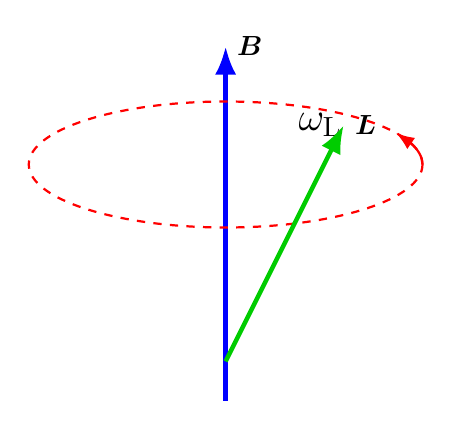
\begin{tikzpicture}[>=Latex]
        % 定義
        \def\Rx{2.5} % 楕円のx半径
        \def\Ry{0.8} % 楕円のy半径
        \def\H{3.5}  % 軸の高さ

        % 座標軸 (B field)
        \draw[blue, ultra thick, ->] (0, -1) -- (0, \H) node[right, black] {$\bm{B}$};
        
        % 歳差運動の軌道 (赤い破線)
        \draw[red, thick, dashed] (0, 2) ellipse ({\Rx} and {\Ry});
        \draw[red, thick, ->] (\Rx, 2) arc (0:30:{\Rx} and {\Ry}); % 回転方向の矢印
        \node at (1.2, 2.5) {\Large $\omega_{\text{L}}$};

        % Angular Momentum Vector L
        % 原点(0,0)から楕円上の点へ
        \draw[green!80!black, ultra thick, ->] (0, -0.5) -- (1.5, 2.5) node[right, black] {$\bm{L}$};
        
    \end{tikzpicture}
    \caption{スピン歳差運動の模式図. スピン演算子 \(\vb*{S}\) が静磁場 \(\vb*{B}\) を軸として, Larmor周波数 \(\omega_{\text{L}}\) で歳差回転運動をする.}
    \label{fig:larmor_precession}
\end{figure}
\chapter{超強結合領域におけるZeemanポラリトンの定量的記述}
\label{chap:zeeman_polariton}

\section{電磁場の量子化}
\section{ベクトルポテンシャルの導入}
クーロンゲージ(\(\nabla \cdot \vb*{A} = 0\))を採用し, 体積 \(V\) のキャビティ内における単一モードの電磁場を考える. 
ベクトルポテンシャル \(\hat{\vb*{A}}(\vb*{r}, t)\) を, キャビティの固有モード関数 \(\vb*{u}(\vb*{r})\) を用いて以下のように量子化する. 
\begin{equation}
    \hat{\vb*{A}}(\vb*{r}) = \sqrt{\frac{\hbar}{2\epsilon_0 \omega_c V}} \left( \hat{a} \vb*{u}(\vb*{r}) + \hat{a}^\dagger \vb*{u}^*(\vb*{r}) \right)
\end{equation}
ここで, \(\hat{a}, \hat{a}^\dagger\) はそれぞれ光子の消滅・生成演算子であり, 交換関係 \([\hat{a}, \hat{a}^\dagger] = 1\) を満たす. \(\omega_c\) はキャビティの共鳴角周波数である. 

\section*{磁場演算子の導出}
磁束密度演算子 \(\hat{\vb*{B}}(\vb*{r})\) は, ベクトルポテンシャルの回転として定義される. 
\begin{equation}
    \hat{\vb*{B}}(\vb*{r}) = \nabla \times \hat{\vb*{A}}(\vb*{r}) = \sqrt{\frac{\hbar}{2\epsilon_0 \omega_c V}} \left( \hat{a} (\nabla \times \vb*{u}(\vb*{r})) + \hat{a}^\dagger (\nabla \times \vb*{u}^*(\vb*{r})) \right)
\end{equation}

\section*{ファラデー配置におけるモード設定}
本実験系(ファラデー配置)に合わせ, 以下の幾何学的条件を設定する. 
\begin{itemize}
    \item 光の伝搬方向(波数ベクトル): \(\vb*{k} \parallel z\)
    \item 静磁場方向: \(\vb*{B}_{\text{DC}} \parallel z\)
    \item キャビティモード: \(z\) 軸方向に定在波を形成する直線偏光モード
\end{itemize}
ここで, 磁場が \(x\) 軸方向に偏光している(\(\vb*{B} \parallel x\))ようなモードを考える. 電磁波の横波性により電場は \(y\) 方向成分を持つため, ベクトルポテンシャルのモード関数を以下のように仮定できる. 
\begin{equation}
    \vb*{u}(\vb*{r}) = u(z) \vb*{e}_y
\end{equation}
これの回転をとると, 
\begin{equation}
    \nabla \times \vb*{u}(\vb*{r}) = \mqty|\vb*{e}_x & \vb*{e}_y & \vb*{e}_z \\ \partial_x & \partial_y & \partial_z \\ 0 & u(z) & 0| = -\frac{d u(z)}{dz} \vb*{e}_x
\end{equation}
となる. スピン集団が配置されている位置(例えば \(z=0\))において磁場が腹(最大振幅)になると仮定し, その局所的な空間微分値を定数 \(C\) (無次元量のオーダー)として扱うと, 
\begin{equation}
    \hat{\vb*{B}} = \sqrt{\frac{\hbar}{2\epsilon_0 \omega_c V}} \frac{k c}{\omega_c} C (\hat{a} + \hat{a}^\dagger) \vb*{e}_x
\end{equation}
のように整理できる. ここで \(\omega_c = c k, c=\frac{1}{\sqrt{\epsilon_0 \mu_0}}\) の関係を用い, すべての定数を真空磁場揺らぎ振幅 \(B_{\text{vac}}\) に押し込めると, 最終的に以下の簡潔な形を得る. 
\begin{equation}
    \hat{\vb*{B}} = B_{\text{vac}} (\hat{a} + \hat{a}^\dagger) \vb*{e}_x, \quad B_{\text{vac}} \equiv C \sqrt{\frac{\hbar \omega_c \mu_0}{2V}}
    \label{eq:B_field}
\end{equation}
これにより, 直線偏光モードの量子化磁場が定義された. 

\section{磁気双極子相互作用}
\section*{ハミルトニアンの定義}
\(N\) 個の局在スピン \(\hat{\vb*{S}}_i\) と量子化磁場 \(\hat{\vb*{B}}\) との相互作用ハミルトニアン \(\hat{\mathcal{H}}_{\text{int}}\) は, ゼーマン・エネルギーの形式(\(-\hat{\boldsymbol{\mu}} \cdot \hat{\vb*{B}}\))で与えられる. 
\begin{equation}
    \hat{\mathcal{H}}_{\text{int}} = - \sum_{i=1}^N \hat{\boldsymbol{\mu}}_i \cdot \hat{\vb*{B}}
\end{equation}
磁気モーメント演算子は \(\hat{\boldsymbol{\mu}}_i = -g_L \mu_B \hat{\vb*{S}}_i\) である(\(g_L\): ランデのg因子, \(\mu_B\): ボーア磁子). 式(\ref{eq:B_field})を代入すると, 磁場が \(x\) 成分のみを持つため, スピンの \(x\) 成分のみが結合する. 
\begin{equation}
    \hat{\mathcal{H}}_{\text{int}} = g_L \mu_B B_{\text{vac}} \sum_{i=1}^N \hat{S}_x^i (\hat{a} + \hat{a}^\dagger)
\end{equation}

\section*{昇降演算子による展開と反回転項}
スピン演算子の \(x\) 成分を昇降演算子 \(\hat{S}_\pm^i = \hat{S}_x^i \pm i \hat{S}_y^i\) を用いて \(\hat{S}_x^i = \frac{1}{2}(\hat{S}_+^i + \hat{S}_-^i)\) と書き換える. 
さらに, 集団スピン演算子 \(\hat{J}_\pm = \sum_i \hat{S}_\pm^i\) を導入する. 
\begin{align}
    \hat{\mathcal{H}}_{\text{int}} &= \frac{g_L \mu_B B_{\text{vac}}}{2} (\hat{J}_+ + \hat{J}_-) (\hat{a} + \hat{a}^\dagger) \\
    &= \frac{g_L \mu_B B_{\text{vac}}}{2} \left[ \underbrace{(\hat{a} \hat{J}_+ + \hat{a}^\dagger \hat{J}_-)}_{\text{回転項}} + \underbrace{(\hat{a} \hat{J}_- + \hat{a}^\dagger \hat{J}_+)}_{\text{反回転項}} \right]
\end{align}
この式変形により, エネルギー保存則を一見破るように見える項(光子生成かつスピン励起 \(\hat{a}^\dagger \hat{J}_+\), およびその逆過程)が自然に出現することがわかる. これらがUSC領域で重要となる反回転項である. 

\section*{Dickeモデルハミルトニアン}
単一スピン当たりの結合定数 \(\hbar g_0 = \frac{1}{2}g_L \mu_B B_{\text{vac}}\) を定義し, 集団増強された結合定数を \(g_{\text{eff}} = g_0 \sqrt{N}\) とおくと, 全ハミルトニアンは以下のように求まる. 
\begin{equation}
    \hat{\mathcal{H}}_{\text{Dicke}} = \hbar \omega_c \hat{a}^\dagger \hat{a} + \hbar \omega_s \hat{J}_z + \frac{\hbar g_{\text{eff}}}{\sqrt{N}} (\hat{a}^\dagger + \hat{a})(\hat{J}_+ + \hat{J}_-) \label{Dicke_Hamiltonian}
\end{equation}
ここで \(\omega_s\) は静磁場によるLarmor周波数である. 
以上より, 直線偏光モードを持つキャビティ場とスピン系の磁気双極子相互作用から, 反回転項を含むDickeハミルトニアンが第一原理的に導出された. 

\section{Holstein-Primakoff変換によるボゾン化}
熱力学的極限(\(N \gg 1\))かつ低励起極限(\(\langle \hat{J}_z \rangle \approx -N/2\))において, 集団スピン演算子に対してHolstein-Primakoff変換を適用し, スピン自由度をボゾン演算子\(\hat{b}, \hat{b}^\dagger\)(マグノン)に写像する. 
\begin{align}
    \hat{J}_+ &\simeq \sqrt{N} \hat{b}^\dagger, \quad \hat{J}_- \simeq \sqrt{N} \hat{b} \\
    \hat{J}_z &= -N/2 + \hat{b}^\dagger \hat{b}
\end{align}
これらをDickeハミルトニアン(式\ref{Dicke_Hamiltonian})に代入し, 定数項を除くと, 以下の2次形式ボゾンハミルトニアン(Hopfieldハミルトニアン)が得られる. 
\begin{equation}
    \hat{\mathcal{H}}_{\text{Hop}} = \hbar \omega_c \hat{a}^\dagger \hat{a} + \hbar \omega_s \hat{b}^\dagger \hat{b} + \hbar g_{\text{eff}} (\hat{a}^\dagger + \hat{a})(\hat{b}^\dagger + \hat{b}) 
    \label{eq:Hopfield}
\end{equation}
式(\ref{eq:Hopfield})は, \(\hat{a}^\dagger \hat{b}^\dagger\)(光子・マグノンの同時生成)および\(\hat{a}\hat{b}\)(同時消滅)を含んでおり, RWAでは記述できない物理現象を示唆している. 

\section{Bogoliubov変換と固有エネルギー}
このハミルトニアン(式\ref{eq:Hopfield})を対角化するために, 一般化されたBogoliubov変換(Hopfield変換)を導入し, 新たな固有演算子(ポラリトン演算子)\(\hat{p}_k\) (\(k=\text{LP, UP}\)) を定義する. 
\begin{equation}
    \hat{p}_k = w_k \hat{a} + x_k \hat{b} + y_k \hat{a}^\dagger + z_k \hat{b}^\dagger
\end{equation}
Heisenbergの運動方程式に基づく行列形式の固有値問題を解くことで, Zeemanポラリトンの分散関係(固有エネルギー \(E_{\pm} = \hbar \Omega_{\pm}\))は以下のように導出される. 
\begin{equation}
    \Omega_{\pm}^2 = \frac{1}{2} \left[ \omega_c^2 + \omega_s^2 \pm \sqrt{(\omega_c^2 - \omega_s^2)^2 + 16 g_{\text{eff}}^2 \omega_c \omega_s} \right]
\end{equation}
この結果は, USC領域において固有振動数が結合強度\(g_{\text{eff}}\)に対して非線形に依存することを示している. 特に\(\Omega_-\)(Lower Polariton)は, Bloch-Siegertシフトを含んだエネルギー準位となる. 
\section{基底状態の量子性}
Dickeモデルにおける真の基底状態(USC真空)\(|G_{\text{USC}}\rangle\) は, ポラリトン消滅演算子に対し \(\hat{p}_k |G_{\text{USC}}\rangle = 0\) を満たす状態として定義される. しかし, 元の粒子演算子(\(\hat{a}, \hat{b}\))に対しては真空ではない. 
すなわち, 
\begin{equation}
    \langle G_{\text{USC}} | \hat{a}^\dagger \hat{a} | G_{\text{USC}} \rangle \neq 0, \quad \langle G_{\text{USC}} | \hat{b}^\dagger \hat{b} | G_{\text{USC}} \rangle \neq 0
\end{equation}
となり, 基底状態においても有限の光子数とマグノン数が存在する(仮想光子の衣をまとう). これは, 系がスクイーズド真空状態にあることを意味し, キャビティ量子電磁力学(Cavity QED)における顕著な量子効果の一つである. 
\include{chapters/appendix_E}
\chapter{H形式とB形式のSRPT発現可能性の違い}
\label{chap:SRPT_realization}

電磁気学において, 磁場を表す物理量には磁束密度\(\vb*{B}\)と磁場の強さ\(\vb*{H}\)の二種類が存在する. これらは真空中では\(\vb*{B} = \mu_0 \vb*{H}\)という単純な比例関係にあるが, GGGのような磁性体内では, その定義と物理的役割に本質的な差異が生じる. \ref{sec:theory_permeability}節でも述べたように, 転送行列法による光学特性の計算においては, どちらの形式を採用するかによって透磁率や境界条件の定義が異なるため, 明確な区別が必要である.
本付録では, 一般の物質中における電磁波の分散関係を導出し, その過程で\(\vb*{B}\)形式と\(\vb*{H}\)形式の違いがどのように分散関係に影響を与えるかを明らかにする. これにより, Zeemanポラリトンの分散関係が両形式でどのように異なるかを理解し, SRPT発現可能性の違いを理論的に裏付ける基礎を提供する.

\section{一般の物質中における電磁波の分散関係の導出}
\subsection{マクスウェル方程式と構成方程式}
電荷密度 \(\rho = 0\) および電流密度 \(\vb*{J} = \vb*{0}\) の一般の物質中におけるMaxwell方程式は以下の通りである. 
\begin{align}
    \nabla \cdot \vb*{D} &= 0 \\
    \nabla \cdot \vb*{B} &= 0 \\
    \nabla \times \vb*{E} &= -\frac{\partial \vb*{B}}{\partial t} \label{eq:Faraday} \\
    \nabla \times \vb*{H} &= \frac{\partial \vb*{D}}{\partial t} \label{eq:Ampere}
\end{align}
ここで, 線形応答を示す等方的な物質を仮定し, 周波数領域における構成方程式を導入する. 
電束密度 \(\vb*{D}\) および磁束密度 \(\vb*{B}\) は, それぞれ電場 \(\vb*{E}\) および磁場 \(\vb*{H}\) と以下の関係にある. 
\begin{align}
    \vb*{D} &= \epsilon_0 \epsilon_r(\omega) \vb*{E} \\
    \vb*{B} &= \mu_0 \mu_r(\omega) \vb*{H}
\end{align}
\(\epsilon_0, \mu_0\) は真空の誘電率と透磁率であり, \(\epsilon_r(\omega), \mu_r(\omega)\) はそれぞれ物質の比誘電率と比透磁率である. 

\subsection{波動方程式の導出}
式(\ref{eq:Faraday})の両辺の回転をとる. 
\begin{equation}
    \nabla \times (\nabla \times \vb*{E}) = -\frac{\partial}{\partial t} (\nabla \times \vb*{B})
\end{equation}
左辺に対し, ベクトル解析の恒等式 \(\nabla \times (\nabla \times \vb*{A}) = \nabla(\nabla \cdot \vb*{A}) - \nabla^2 \vb*{A}\) を適用する. 均質な媒質中では \(\nabla \cdot \vb*{E} = 0\) となるため, 左辺は \(-\nabla^2 \vb*{E}\) となる. 
右辺に対し, \(\vb*{B} = \mu_0 \mu_r \vb*{H}\) および式(\ref{eq:Ampere})を代入する. 
\begin{align}
    -\nabla^2 \vb*{E} &= -\mu_0 \mu_r \frac{\partial}{\partial t} (\nabla \times \vb*{H}) \nonumber \\
    &= -\mu_0 \mu_r \frac{\partial}{\partial t} \left( \epsilon_0 \epsilon_r \frac{\partial \vb*{E}}{\partial t} \right) \nonumber \\
    &= -\epsilon_0 \mu_0 \epsilon_r \mu_r \frac{\partial^2 \vb*{E}}{\partial t^2}
\end{align}
真空中の光速 \(c = 1/\sqrt{\epsilon_0 \mu_0}\) を用いて整理すると, 以下の波動方程式が得られる. 
\begin{equation}
    \left( \nabla^2 - \frac{\epsilon_r \mu_r}{c^2} \frac{\partial^2}{\partial t^2} \right) \vb*{E}(\vb*{r}, t) = 0
\end{equation}

\subsection{平面波解と分散関係}
単色平面波解 \(\vb*{E}(\vb*{r}, t) = \vb*{E}_0 e^{i(\vb*{k} \cdot \vb*{r} - \omega t)}\) を仮定し, 波動方程式に代入する. 
空間微分 \(\nabla \to i\vb*{k}\), 時間微分 \(\partial/\partial t \to -i\omega\) の置き換えにより, 
\begin{equation}
    -k^2 \vb*{E}_0 + \frac{\epsilon_r \mu_r}{c^2} \omega^2 \vb*{E}_0 = 0
\end{equation}
非自明な解(\(\vb*{E}_0 \neq \vb*{0}\))が存在するための条件として, 以下の分散関係式が得られる. 
\begin{equation}
    k^2 = \epsilon_r(\omega) \mu_r(\omega) \frac{\omega^2}{c^2}
\end{equation}
あるいは, 屈折率 \(n(\omega) = \sqrt{\epsilon_r(\omega) \mu_r(\omega)}\) を用いて, 
\begin{equation}
    \frac{ck}{\omega} = \sqrt{\epsilon_r(\omega) \mu_r(\omega)}
    \label{eq:dispersion_general}
\end{equation}
と表される. この式(\ref{eq:dispersion_general})が, 一般の物質中における光子(ポラリトン)の分散関係の基礎式である. 
本研究で扱うZeemanポラリトンの場合, \(\mu_r(\omega)\) の定義(B形式またはH形式)によって右辺の周波数依存性が変化し, 分散曲線の形状に図\ref{fig:dispersion_relation}のように決定的な影響を与える. 

\begin{figure}
    \centering
    \includegraphics[width=1.0\textwidth]{figures/dispersion_relation.png}
    \caption{一般の物質中における光子(ポラリトン)の分散関係. 比誘電率 \(\epsilon_r(\omega)\) および比透磁率 \(\mu_r(\omega)\) の周波数依存性により, 分散曲線の形状が決定される. Zeemanポラリトンの場合, \(\mu_r(\omega)\) の定義(B形式またはH形式)によって分散関係が変化する. ただし, \(\omega_0\)は\(\omega_{\text{cav}}=\omega_{\text{EPR}}\)を満たす共鳴周波数}
    \label{fig:dispersion_relation}
\end{figure}
\chapter{相互作用描像・線形応答理論に基づく磁気感受率の導出}
\label{chap:Kubo_formula_derivation}

GGGの磁気光学的応答(透過率や反射率)を計算するためには, 物質の動的磁気感受率\(\chi(\omega)\)を知る必要がある. これは, 外部からの微弱な振動磁場に対する磁化の応答として定義され, 量子統計力学における線形応答理論(Linear Response Theory)を用いて厳密に導出される. 本節では, 久保公式\(^{\cite{Kubo1957}}\)の導出過程を相互作用描像を用いて詳細に示す. 

\section{Liouville方程式と相互作用描像}
\subsection{Liouville-von Neumann方程式の導出}

密度演算子(密度行列)\(\hat{\rho}(t)\)の時間発展方程式であるLiouville-von Neumann方程式を, Schrödinger方程式より導出する. 
ある量子系が, 確率\(p_n\)で純粋状態\(|\psi_n(t)\rangle\)にある混合状態を考える. このとき, 密度演算子は以下のように定義される. 

\begin{equation}
\hat{\rho}(t) = \sum_n p_n |\psi_n(t)\rangle \langle \psi_n(t)|
\end{equation}

ここで, 確率\(p_n\)は時間的に変化しない(\(\dot{p}_n = 0\))と仮定する. これは, 外部環境とのエネルギーや粒子のやり取りによる緩和過程を含まない, 閉じた系におけるユニタリ発展を記述するためである. 
\(\hat{\rho}(t)\)を時間\(t\)で微分すると, Leibniz則より以下のようになる. 

\begin{equation}
\frac{\partial \hat{\rho}(t)}{\partial t} = \sum_n p_n \left[ \left( \frac{\partial}{\partial t} |\psi_n(t)\rangle \right) \langle \psi_n(t)| + |\psi_n(t)\rangle \left( \frac{\partial}{\partial t} \langle \psi_n(t)| \right) \right]
\label{eq:rho_dot}
\end{equation}

一方, 状態ベクトル\(|\psi_n(t)\rangle\)は時間依存Schrödinger方程式に従う. 

\begin{equation}
i\hbar \frac{\partial}{\partial t} |\psi_n(t)\rangle = \hat{\mathcal{H}}(t) |\psi_n(t)\rangle
\end{equation}

この式の両辺を\(i\hbar\)で割り, ケットベクトルの時間微分を得る. 

\begin{equation}
\frac{\partial}{\partial t} |\psi_n(t)\rangle = \frac{1}{i\hbar} \hat{\mathcal{H}}(t) |\psi_n(t)\rangle = -\frac{i}{\hbar} \hat{\mathcal{H}}(t) |\psi_n(t)\rangle
\end{equation}

また, エルミート共役をとることで, ブラベクトルの時間微分が得られる(ハミルトニアンのエルミート性 \(\hat{\mathcal{H}}^\dagger = \hat{\mathcal{H}}\) を用いる). 

\begin{equation}
-i\hbar \frac{\partial}{\partial t} \langle \psi_n(t)| = \langle \psi_n(t)| \hat{\mathcal{H}}(t) \quad \longrightarrow \quad \frac{\partial}{\partial t} \langle \psi_n(t)| = \frac{i}{\hbar} \langle \psi_n(t)| \hat{\mathcal{H}}(t)
\end{equation}

これらを式(\ref{eq:rho_dot})に代入すると, 

\begin{align}
\frac{\partial \hat{\rho}(t)}{\partial t} &= \sum_n p_n \left[ \left( -\frac{i}{\hbar} \hat{\mathcal{H}}(t) |\psi_n(t)\rangle \right) \langle \psi_n(t)| + |\psi_n(t)\rangle \left( \frac{i}{\hbar} \langle \psi_n(t)| \hat{\mathcal{H}}(t) \right) \right] \nonumber \\
&= -\frac{i}{\hbar} \hat{\mathcal{H}}(t) \left( \sum_n p_n |\psi_n(t)\rangle \langle \psi_n(t)| \right) + \frac{i}{\hbar} \left( \sum_n p_n |\psi_n(t)\rangle \langle \psi_n(t)| \right) \hat{\mathcal{H}}(t) \nonumber \\
&= -\frac{i}{\hbar} \left( \hat{\mathcal{H}}(t)\hat{\rho}(t) - \hat{\rho}(t)\hat{\mathcal{H}}(t) \right) \nonumber \\
&= -\frac{i}{\hbar} [\hat{\mathcal{H}}(t), \hat{\rho}(t)]
\end{align}

整理して, 以下のLiouville-von Neumann方程式を得る. 

\begin{equation}
i\hbar \frac{\partial \hat{\rho}(t)}{\partial t} = [\hat{\mathcal{H}}(t), \hat{\rho}(t)]
\end{equation}

この方程式は, 古典力学におけるLiouville方程式の量子力学的対応物であり, 量子状態の確率分布の時間発展を記述する基礎方程式である. \\
\(\hat{\mathcal{H}}(t)\)は, 時間的に変化しない非摂動系のハミルトニアン\(\hat{\mathcal{H}}_0\)と, 時刻\(t_0\)以降に印加される外部摂動\(\hat{\mathcal{H}}'(t)\)の和で表される. 
\begin{equation}
\hat{\mathcal{H}}(t) = \hat{\mathcal{H}}_0 + \hat{\mathcal{H}}'(t)
\end{equation}
外部振動場\(\vb*{h}(t)\)に対するZeemanエネルギーを摂動とすると, \(\hat{\mathcal{H}}'(t) = - \hat{\vb*{M}} \cdot \vb*{h}(t)\)である(\(\hat{\vb*{M}}\)は全磁化演算子). 

ここで, 計算の見通しを良くするために, Schrödinger描像から相互作用描像への変換を行う. 相互作用描像における密度演算子\(\rho_I(t)\)および任意の演算子\(\hat{A}_I(t)\)は以下のように定義される:

\begin{align}
\rho_I(t) &= e^{i\hat{\mathcal{H}}_0 t / \hbar} \rho(t) e^{-i\hat{\mathcal{H}}_0 t / \hbar} \\
\hat{A}_I(t) &= e^{i\hat{\mathcal{H}}_0 t / \hbar} \hat{A} e^{-i\hat{\mathcal{H}}_0 t / \hbar}
\end{align}

Liouville方程式に\(\rho(t) = e^{-i\hat{\mathcal{H}}_0 t / \hbar} \rho_I(t) e^{i\hat{\mathcal{H}}_0 t / \hbar}\)を代入して整理すると, 相互作用描像における時間発展方程式は, 摂動項\(\hat{\mathcal{H}}'_I(t)\)のみを含む形となる:

\begin{equation}
i\hbar \frac{\partial \rho_I(t)}{\partial t} = [\hat{\mathcal{H}}'_I(t), \rho_I(t)]
\end{equation}

\section{摂動展開と線形応答}

系は\(t=-\infty\)において熱平衡状態\(\rho_{\text{eq}} = e^{-\beta \hat{\mathcal{H}}_0} / Z\)にあったと仮定する(\(\beta = 1/k_B T\)). 摂動が微弱であるとして, \(\rho_I(t)\)を\(\hat{\mathcal{H}}'\)について級数展開し, 一次の項までをとる(線形近似). 

\begin{gather}
\rho_I(t) = \rho_0 + \Delta \rho_I(t) \\
i\hbar \frac{\partial \Delta \rho_I(t)}{\partial t} \approx [\hat{\mathcal{H}}'_I(t), \rho_0]
\end{gather}

これを積分形に直すと, 

\begin{equation}
\Delta \rho_I(t) = -\frac{i}{\hbar} \int_{-\infty}^t dt' [\hat{\mathcal{H}}'_I(t'), \rho_0]
\end{equation}

シュレーディンガー描像における密度行列の変化\(\Delta \rho(t)\)は, 逆変換により以下のように得られる:

\begin{equation}
\Delta \rho(t) = e^{-i\hat{\mathcal{H}}_0 t / \hbar} \Delta \rho_I(t) e^{i\hat{\mathcal{H}}_0 t / \hbar} = -\frac{i}{\hbar} \int_{-\infty}^t dt' e^{-i\hat{\mathcal{H}}_0 t / \hbar} [\hat{\mathcal{H}}'_I(t'), \rho_0] e^{i\hat{\mathcal{H}}_0 t / \hbar}
\end{equation}

\section{久保公式(Kubo Formula)の導出}

観測量である磁化\(\hat{M}_\alpha\)(\(\alpha = x, y, z\))の期待値の変化\(\Delta \langle M_\alpha(t) \rangle\)は, トレースを用いて計算される. 

\begin{equation}
\Delta \langle M_\alpha(t) \rangle = \text{Tr}(\Delta \rho(t) \hat{M}_\alpha)
\end{equation}

トレースの巡回不変性(\(\text{Tr}(ABC) = \text{Tr}(BCA)\))を利用して式を変形する. 

\begin{align}
\Delta \langle M_\alpha(t) \rangle &= -\frac{i}{\hbar} \int_{-\infty}^t dt' \text{Tr}\left( [\hat{\mathcal{H}}'_I(t'), \rho_0] e^{i\hat{\mathcal{H}}_0 t / \hbar} \hat{M}_\alpha e^{-i\hat{\mathcal{H}}_0 t / \hbar} \right) \nonumber \\
&= -\frac{i}{\hbar} \int_{-\infty}^t dt' \text{Tr}\left( [\hat{\mathcal{H}}'_I(t'), \rho_0] \hat{M}_{\alpha, I}(t) \right) \nonumber \\
&= -\frac{i}{\hbar} \int_{-\infty}^t dt' \text{Tr}\left( \rho_0 [\hat{M}_{\alpha, I}(t), \hat{\mathcal{H}}'_I(t')] \right) \quad (\because \text{Tr}([A, \rho]B) = \text{Tr}(\rho [B, A]))
\end{align}

外部磁場が\(\vb*{h}(t')\)として\(\hat{M}_\beta\)成分に結合している場合, \(\hat{\mathcal{H}}'_I(t') = - \hat{M}_{\beta, I}(t') h_\beta(t')\)であるから, 

\begin{equation}
\Delta \langle M_\alpha(t) \rangle = \int_{-\infty}^t dt' \frac{i}{\hbar} \langle [\hat{M}_{\alpha, I}(t), \hat{M}_{\beta, I}(t')] \rangle_0 h_\beta(t')
\end{equation}

ここで, \(\langle \dots \rangle_0 = \text{Tr}(\rho_0 \dots)\)は平衡状態でのアンサンブル平均を表す. 応答関数\(\phi_{\alpha\beta}(t-t')\)を以下のように定義すると, これが久保公式である. 

\begin{equation}
\phi_{\alpha\beta}(t-t') = \frac{i}{\hbar} \theta(t-t') \langle [\hat{M}_\alpha(t), \hat{M}_\beta(t')] \rangle_0
\end{equation}

\(\theta(t)\)は因果律を表す階段関数である. 周波数領域での感受率\(\chi_{\alpha\beta}(\omega)\)は, この応答関数のフーリエ変換として与えられる. 

\begin{equation}
\chi_{\alpha\beta}(\omega) = \int_0^\infty dt e^{i\omega t} \phi_{\alpha\beta}(t)
\end{equation}

この式は, \textbf{「外部磁場に対する巨視的な磁化の応答(非平衡過程)は, 熱平衡状態における磁化の量子力学的な揺らぎ(交換関係の相関関数)によって完全に記述される」}という揺動散逸定理の物理的基礎を与えている. 
\chapter{磁気感受率テンソルの計算}
\label{chap:appendix_F}
本付録では, \ref{sec:linear_response}節で導出した磁気感受率テンソルの計算において, Zeeman準位の重ね合わせ準位による厳密な固有状態を用いて詳細に計算した結果を示す. 具体的には, 外部磁場下での\(\text{Gd}^{3+}\)イオンのスピン状態をZeeman準位\(\ket{m_S}\) (\(m_S = -7/2, -5/2, \ldots, 7/2\)) の線形結合として表現し, 磁気感受率テンソル\(\chi_{ij} (\omega)\)を求めた. これにより, 各固有状態がどのようなZeeman準位の重ね合わせで構成されているかを明らかにした.\\

固有状態\(\ket{\psi_n}\)は, スピン\(s\)の磁気量子数\(m\)を用いて, 各準位\(\ket{m}\)の重ね合わせとして表される. すなわち, 
\begin{equation}
  \ket{\psi_n} = \sum_{m} c_{n,m} \ket{m} (m = -s, -s+1, \ldots, s-1, s)
\end{equation} 
である.

磁気モーメント演算子\(\hat{d}_{i}\)はスピン演算子\(\hat{S}_{i}\)を用いて以下のように表される.
\begin{equation}
\langle m | \hat{d}_{i,j} | m' \rangle = \mu_{B} g \langle m | \hat{S}_{i,j} | m' \rangle
\end{equation}

また, スピン演算子は昇降演算子\(\hat{S}_{\pm}\)を用いて以下のように表される.
\begin{equation*}
\hat{S}_{x} = \frac{1}{2} (\hat{S}_{+} + \hat{S}_{-}), \quad \hat{S}_{y} = \frac{1}{2i} (\hat{S}_{+} - \hat{S}_{-}), \quad \hat{S}_{z} = m
\end{equation*}
以上より, 

\begin{equation}
\langle m | \hat{d}_{x} | m' \rangle = \frac{\mu_{B} g \hbar}{2} (\delta_{m', m-1} \sqrt{(s + m)(s - m + 1)} + \delta_{m', m+1} \sqrt{(s - m)(s + m + 1)} )
\end{equation}

\begin{equation}
\langle m | \hat{d}_{y} | m' \rangle = \frac{\mu_{B} g \hbar}{2i} (\delta_{m', m-1} \sqrt{(s + m)(s - m + 1)} - \delta_{m', m+1} \sqrt{(s - m)(s + m + 1)} )
\end{equation}

計算の見通しを良くするために, 次のように\(F_{\pm}, K\)を定義する.

\begin{align}
F_{+} &= \sum_{m} C_{n,m} C_{n',m-1} \sqrt{(s + m)(s - m + 1)}, \\ 
F_{-} &= \sum_{m} C_{n,m} C_{n',m+1}\sqrt{(s - m)(s + m + 1)}, \\
F_z &= \sum_{m} C_{n,m} C_{n',m} m, \\
K &= \left(\frac{\mu_{B} g \hbar}{2}\right)^2 
\end{align}

これらを用いると, 磁気モーメント演算子の各成分は以下のように表される.
\begin{align}
\langle \psi_{n} | \hat{d}_{x} | \psi_{n'} \rangle &= K (F_{+} + F_{-}), \\
\langle \psi_{n} | \hat{d}_{y} | \psi _{n'} \rangle &= K (F_{+} - F_{-}), \\
\langle \psi_{n} | \hat{d}_{z} | \psi_{n'} \rangle &= K F_z 
\end{align}

エルミート演算子の性質より, \(\langle \psi_{n'} | \hat{d}_{i} | \psi_{n} \rangle = \langle \psi_{n} | \hat{d}_{i} | \psi_{n'} \rangle^{*}\)であることに注意すると, 
\begin{align}
\langle \psi_{n'} | \hat{d}_{x} | \psi_{n} \rangle &= \langle \psi_{n} | \hat{d}_{x} | \psi_{n'} \rangle = K (F_{+} + F_{-}), \\
\langle \psi_{n'} | \hat{d}_{y} | \psi _{n} \rangle &= \langle \psi_{n} | \hat{d}_{y} | \psi_{n'} \rangle = K (F_{+} - F_{-}), \\
\langle \psi_{n'} | \hat{d}_{z} | \psi_{n} \rangle &= \langle \psi_{n} | \hat{d}_{z} | \psi_{n'} \rangle = K F_z
\end{align}

以上より, 磁気感受率テンソルの各成分は以下のように表される.
\begin{align}
\chi_{xx}(\omega) &= - \frac{N \mu_{0}}{\hbar} \sum_{n, n'} P_{n} \{ \frac{K^2 (F_{+} + F_{-})^2}{\omega + i \gamma - \Delta \omega} - \frac{K^2 (F_{+} + F_{-})^2}{\omega + i \gamma + \Delta \omega} \}, \\
\chi_{yy}(\omega) &= - \frac{N \mu_{0}}{\hbar} \sum_{n, n'} P_{n} \{ \frac{K^2 (F_{+} - F_{-})^2}{\omega + i \gamma - \Delta \omega} - \frac{K^2 (F_{+} - F_{-})^2}{\omega + i \gamma + \Delta \omega} \}, \\
\chi_{zz}(\omega) &= - \frac{N \mu_{0}}{\hbar} \sum_{n, n'} P_{n} \{ \frac{K^2 F_z^2}{\omega + i \gamma - \Delta \omega} - \frac{K^2 F_z^2}{\omega + i \gamma + \Delta \omega} \}, \\
\chi_{xy}(\omega) &= - \frac{N \mu_{0}}{\hbar} \sum_{n, n'} P_{n} \{ \frac{K^2 (F_{+} + F_{-})(F_{+} - F_{-})}{\omega + i \gamma - \Delta \omega} - \frac{K^2 (F_{+} + F_{-})(F_{+} - F_{-})}{\omega + i \gamma + \Delta \omega} \}, \\
\chi_{yx}(\omega) &= \frac{N \mu_{0}}{\hbar} \sum_{n, n'} P_{n} \{ \frac{K^2 (F_{+} - F_{-})(F_{+} + F_{-})}{\omega + i \gamma - \Delta \omega} - \frac{K^2 (F_{+} - F_{-})(F_{+} + F_{-})}{\omega + i \gamma + \Delta \omega} \}\notag \\ &= -\chi_{xy}(\omega), \\
\chi_{xz}(\omega) &= - \frac{N \mu_{0}}{\hbar} \sum_{n, n'} P_{n} \{ \frac{K^2 (F_{+} + F_{-})F_z}{\omega + i \gamma - \Delta \omega} - \frac{K^2 (F_{+} + F_{-})F_z}{\omega + i \gamma + \Delta \omega} \}, \\
\chi_{yz}(\omega) &= - \frac{N \mu_{0}}{\hbar} \sum_{n, n'} P_{n} \{ \frac{K^2 (F_{+} - F_{-})F_z}{\omega + i \gamma - \Delta \omega} - \frac{K^2 (F_{+} - F_{-})F_z}{\omega + i \gamma + \Delta \omega} \}
\end{align}
\chapter{Faraday配置における磁気感受率テンソルの円偏光基底への変換}
\label{chap:appendix_circular}
Kritzellらの実験では等方性物質であるGGGを用いて, Faraday配置(磁場 \(\vb*{B} \parallel \vb*{k} \parallel z\))で透過スペクトルを測定している.\(^{\cite{Kritzell2024}}\) この配置では, 円偏光基底における磁気感受率テンソル\(\chi_{\pm}\)が重要となる. そこで, 直線偏光基底での磁気感受率テンソル\(\chi_{ij}\)を, 円偏光基底に変換する方法を以下に示す.

\section{問題設定}
Faraday配置(磁場 \(\vb*{B} \parallel \vb*{k} \parallel z\))における, 等方性媒質(または立方晶系)の線形応答を考える. 
直線偏光基底(デカルト座標系 \(\{x, y, z\}\))における磁気感受率テンソル \(\vb*{\chi}_{\text{lin}}\) は, 磁気光学効果により以下の反対称成分を持つ. 

\begin{equation}
    \vb*{\chi}_{\text{lin}} = 
    \begin{pmatrix}
    \chi_{xx} & \chi_{xy} & 0 \\
    -\chi_{xy} & \chi_{xx} & 0 \\
    0 & 0 & \chi_{zz}
    \end{pmatrix}
\end{equation}
ここで, \(\chi_{xx}\) は対角成分, \(\chi_{xy}\) はジャイロトロピックな非対角成分を表す. 

\section{基底変換行列 (Unitary Transformation)}
直線偏光基底から円偏光基底への変換を考える. 
ここでは, 右円偏光 (\(\sigma_+\)) および左円偏光 (\(\sigma_-\)) の基底ベクトルを, 標準的なジョーンズベクトルの定義(時間依存性 \(e^{-i\omega t}\))に従い以下のように定義する. 
\begin{align}
    \hat{\vb*{e}}_+ &= \frac{1}{\sqrt{2}}(\hat{\vb*{x}} - i\hat{\vb*{y}}) \\
    \hat{\vb*{e}}_- &= \frac{1}{\sqrt{2}}(\hat{\vb*{x}} + i\hat{\vb*{y}})
\end{align}
このとき, 基底変換行列(ユニタリ行列)\(U\) は以下のように与えられる. 
\begin{equation}
    U = \frac{1}{\sqrt{2}}
    \begin{pmatrix}
    1 & i & 0 \\
    1 & -i & 0 \\
    0 & 0 & \sqrt{2}
    \end{pmatrix}
\end{equation}
この行列 \(U\) は, 直線偏光基底のベクトル \(\vb*{v}_{\text{lin}}\) を円偏光基底 \(\vb*{v}_{\text{circ}}\) へ変換する(\(\vb*{v}_{\text{circ}} = U \vb*{v}_{\text{lin}}\)). 

\section{円偏光基底でのテンソル表現}
テンソルの変換則 \(\vb*{\chi}_{\text{circ}} = U \vb*{\chi}_{\text{lin}} U^{-1}\) (ユニタリ性より \(U^{-1} = U^{\dagger}\))に従い計算を行う. 

\begin{align}
    \vb*{\chi}_{\text{circ}} &= U \vb*{\chi}_{\text{lin}} U^{\dagger} \notag \\
    &= \frac{1}{2}
    \begin{pmatrix}
    1 & i & 0 \\
    1 & -i & 0 \\
    0 & 0 & \sqrt{2}
    \end{pmatrix}
    \begin{pmatrix}
    \chi_{xx} & \chi_{xy} & 0 \\
    -\chi_{xy} & \chi_{xx} & 0 \\
    0 & 0 & \chi_{zz}
    \end{pmatrix}
    \begin{pmatrix}
    1 & 1 & 0 \\
    -i & i & 0 \\
    0 & 0 & \sqrt{2}
    \end{pmatrix} \notag \\
    &= \frac{1}{2}
    \begin{pmatrix}
    \chi_{xx}-i\chi_{xy} & \chi_{xy}+i\chi_{xx} & 0 \\
    \chi_{xx}+i\chi_{xy} & -\chi_{xy}+i\chi_{xx} & 0 \\
    0 & 0 & 2\chi_{zz}
    \end{pmatrix}
    \begin{pmatrix}
    1 & 1 & 0 \\
    -i & i & 0 \\
    0 & 0 & \sqrt{2}
    \end{pmatrix} \notag \\
    &= 
    \begin{pmatrix}
    \chi_{xx} - i\chi_{xy} & 0 & 0 \\
    0 & \chi_{xx} + i\chi_{xy} & 0 \\
    0 & 0 & \chi_{zz}
    \end{pmatrix}
\end{align}

\section{結論と物理的解釈}
計算の結果, 円偏光基底において磁気感受率テンソルは\textbf{対角化}されることが示された. 
\begin{equation}
    \vb*{\chi}_{\text{circ}} = 
    \begin{pmatrix}
    \chi_+ & 0 & 0 \\
    0 & \chi_- & 0 \\
    0 & 0 & \chi_{zz}
    \end{pmatrix}
\end{equation}
ここで, 対角成分(固有値)は以下のように定義される. 
\begin{equation}
    \chi_{\pm} = \chi_{xx} \mp i\chi_{xy}
\end{equation}
これは, Faraday配置において円偏光がこの系の\textbf{固有モード (Eigenmodes)} であることを意味する. 

\nocite{*}
\bibliographystyle{naturemag} % 参考文献のスタイルを指定
\bibliography{bib/reference} % .bibファイルのパスを正しく指定

\end{document}